% Options for packages loaded elsewhere
\PassOptionsToPackage{unicode}{hyperref}
\PassOptionsToPackage{hyphens}{url}
\PassOptionsToPackage{dvipsnames,svgnames,x11names}{xcolor}
\PassOptionsToPackage{space}{xeCJK}
\documentclass[
  11pt,
  a4paper,
  oneside,
  openany]{report}
\usepackage{xcolor}
\usepackage[top=25mm,bottom=22mm,left=22mm,right=22mm,headheight=15pt,headsep=7mm]{geometry}
\usepackage{amsmath,amssymb}
\setcounter{secnumdepth}{5}
\usepackage{iftex}
\ifPDFTeX
  \usepackage[T1]{fontenc}
  \usepackage[utf8]{inputenc}
  \usepackage{textcomp} % provide euro and other symbols
\else % if luatex or xetex
  \usepackage{unicode-math} % this also loads fontspec
  \defaultfontfeatures{Scale=MatchLowercase}
  \defaultfontfeatures[\rmfamily]{Ligatures=TeX,Scale=1}
\fi
\usepackage{lmodern}
\ifPDFTeX\else
  % xetex/luatex font selection
  \setmainfont[Path=/Users/zhli/.cache/codex-runtimes/codex-primary-runtime/dependencies/native/libreoffice-headless/libreoffice/LibreOfficeDev.app/Contents/Resources/fonts/truetype/,BoldFont=LiberationSerif-Bold.ttf,ItalicFont=LiberationSerif-Italic.ttf,BoldItalicFont=LiberationSerif-BoldItalic.ttf]{LiberationSerif-Regular.ttf}
  \ifXeTeX
    \usepackage{xeCJK}
    \setCJKmainfont[Path=/usr/local/texlive/2026/texmf-dist/fonts/opentype/public/fandol/,Extension=.otf,UprightFont=*-Regular,BoldFont=*-Bold,ItalicFont=FandolKai-Regular]{FandolSong}
    \setCJKsansfont[Path=/usr/local/texlive/2026/texmf-dist/fonts/opentype/public/fandol/,Extension=.otf,UprightFont=*-Regular,BoldFont=*-Bold,ItalicFont=FandolKai-Regular]{FandolHei}
    \setCJKmonofont[Path=/usr/local/texlive/2026/texmf-dist/fonts/opentype/public/fandol/,Extension=.otf,UprightFont=*-Regular,BoldFont=*-Bold,ItalicFont=FandolKai-Regular]{FandolSong}
  \fi
  \ifLuaTeX
    \usepackage[]{luatexja-fontspec}
    \setmainjfont[Path=/usr/local/texlive/2026/texmf-dist/fonts/opentype/public/fandol/,Extension=.otf,UprightFont=*-Regular,BoldFont=*-Bold,ItalicFont=FandolKai-Regular]{FandolSong}
  \fi
\fi
% Use upquote if available, for straight quotes in verbatim environments
\IfFileExists{upquote.sty}{\usepackage{upquote}}{}
\IfFileExists{microtype.sty}{% use microtype if available
  \usepackage[]{microtype}
  \UseMicrotypeSet[protrusion]{basicmath} % disable protrusion for tt fonts
}{}
\usepackage{setspace}
\makeatletter
\@ifundefined{KOMAClassName}{% if non-KOMA class
  \IfFileExists{parskip.sty}{%
    \usepackage{parskip}
  }{% else
    \setlength{\parindent}{0pt}
    \setlength{\parskip}{6pt plus 2pt minus 1pt}}
}{% if KOMA class
  \KOMAoptions{parskip=half}}
\makeatother
\usepackage{longtable,booktabs,array}
\usepackage{calc} % for calculating minipage widths
% Correct order of tables after \paragraph or \subparagraph
\usepackage{etoolbox}
\makeatletter
\patchcmd\longtable{\par}{\if@noskipsec\mbox{}\fi\par}{}{}
\makeatother
% Allow footnotes in longtable head/foot
\IfFileExists{footnotehyper.sty}{\usepackage{footnotehyper}}{\usepackage{footnote}}
\makesavenoteenv{longtable}
\setlength{\emergencystretch}{3em} % prevent overfull lines
\providecommand{\tightlist}{%
  \setlength{\itemsep}{0pt}\setlength{\parskip}{0pt}}
\usepackage{amsmath,amssymb,booktabs,longtable,array,graphicx,caption,fancyhdr,xcolor,float,titlesec,tcolorbox,enumitem,needspace}
\definecolor{NoteBlue}{HTML}{24364B}
\definecolor{NoteTeal}{HTML}{20667C}
\definecolor{NotePale}{HTML}{EFF5F7}
\setlength{\emergencystretch}{3em}
\setlength{\parindent}{2em}
\setlength{\parskip}{0.28em}
\setlist{nosep,leftmargin=2em,topsep=0.3em}
\setcounter{tocdepth}{1}
\renewcommand{\contentsname}{目录}
\renewcommand{\figurename}{图}
\renewcommand{\tablename}{表}
\titleformat{\chapter}[hang]{\sffamily\bfseries\color{NoteBlue}\fontsize{21}{27}\selectfont}{第\ \thechapter\ 章}{0.8em}{}
\titleformat{name=\chapter,numberless}[hang]{\sffamily\bfseries\color{NoteBlue}\fontsize{21}{27}\selectfont}{}{0pt}{}
\titlespacing*{\chapter}{0pt}{4pt}{24pt}
\titleformat{\section}{\sffamily\bfseries\color{NoteBlue}\fontsize{14}{20}\selectfont}{\thesection}{0.7em}{}
\titleformat{\subsection}{\sffamily\bfseries\color{NoteBlue}\fontsize{11.5}{16}\selectfont}{\thesubsection}{0.7em}{}
\titlespacing*{\section}{0pt}{1.1em}{0.45em}
\titlespacing*{\subsection}{0pt}{0.8em}{0.3em}
\captionsetup{font=small,labelfont=bf,justification=justified,singlelinecheck=false,skip=6pt}
\setlength{\intextsep}{9pt}
\pagestyle{fancy}
\fancyhf{}
\fancyhead[L]{\small\color{NoteBlue}探测器中的信号形成}
\fancyhead[R]{\small\color{NoteBlue}\nouppercase{\leftmark}}
\fancyfoot[C]{\small\thepage}
\renewcommand{\headrulewidth}{0.3pt}
\renewcommand{\chaptermark}[1]{\markboth{\thechapter\quad #1}{}}
\fancypagestyle{plain}{\fancyhf{}\fancyfoot[C]{\small\thepage}\renewcommand{\headrulewidth}{0pt}}
\newtcolorbox{notebox}[1]{colback=NotePale,colframe=NoteTeal,colbacktitle=NoteTeal,coltitle=white,title=#1,fonttitle=\sffamily\bfseries,boxrule=0.4pt,arc=1mm,left=8pt,right=8pt,top=5pt,bottom=5pt,before skip=9pt,after skip=9pt}
\newcommand{\sourcepages}[1]{{\small\color{NoteTeal}原稿对应：第 #1 页}\par\vspace{8pt}}
\newcommand{\fig}[4]{\begin{figure}[H]\centering\includegraphics[width=#2\linewidth]{../l2_curated_figures/#1.pdf}\caption{#3}\label{fig:#1}\end{figure}}
\numberwithin{equation}{chapter}
\AtBeginDocument{\renewcommand{\maketitle}{}}
\usepackage{bookmark}
\IfFileExists{xurl.sty}{\usepackage{xurl}}{} % add URL line breaks if available
\urlstyle{same}
\hypersetup{
  pdftitle={探测器中的信号形成（L2）},
  pdfauthor={探测器信号形成课程讲义},
  colorlinks=true,
  linkcolor={NoteTeal},
  filecolor={Maroon},
  citecolor={Blue},
  urlcolor={NoteTeal},
  pdfcreator={LaTeX via pandoc}}

\title{探测器中的信号形成（L2）}
\author{探测器信号形成课程讲义}
\date{}

\begin{document}
\maketitle

\setstretch{1.17}
\begin{titlepage}
\thispagestyle{empty}
\vspace*{20mm}
{\sffamily\color{NoteTeal}\large DETECTOR SIGNAL FORMATION\par}
\vspace{13mm}
{\sffamily\bfseries\color{NoteBlue}\fontsize{29}{38}\selectfont 探测器中的信号形成\par}
\vspace{7mm}
{\sffamily\Large 电荷沉积、载流子输运与器件信号\par}
\vspace{10mm}
{\large 第 2 册\quad 中文讲义\par}
\vspace{22mm}
\noindent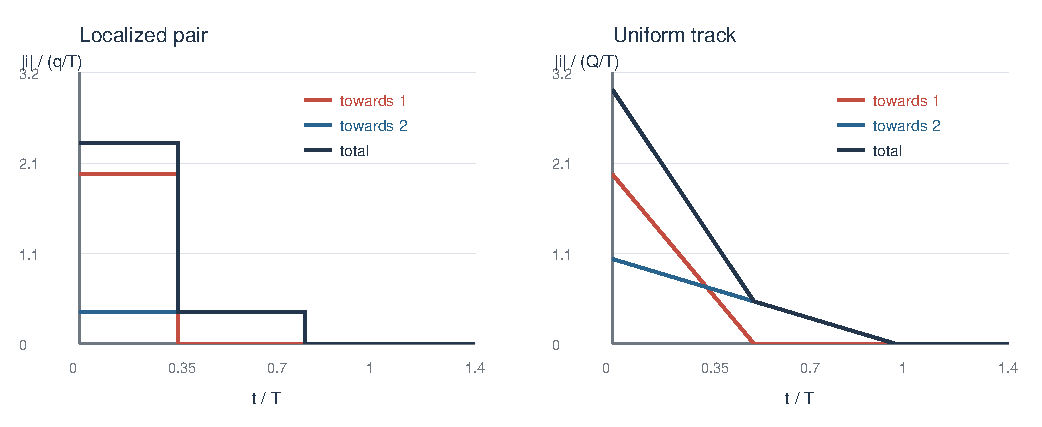
\includegraphics[width=0.94\linewidth]{../l2_curated_figures/parallel_pulses.pdf}
\vfill
{\color{NoteBlue}高年级本科与研究生课程\par}
\end{titlepage}
\pagenumbering{roman}

\chapter*{记号与参考方向}\label{ux8bb0ux53f7ux4e0eux53c2ux8003ux65b9ux5411}
\addcontentsline{toc}{chapter}{记号与参考方向}

运动电荷的真实轨迹由偏置场和输运决定；电极对这段运动的响应由权重场决定。对读出电极
\(k\)，令其辅助电势为 1，其余电极为
0，并移去待测电荷和独立体空间电荷，得到无量纲权重势
\(\varphi_{w,k}\)。在线性、固定介电结构中，采用

\[
\mathbf E_{w,k}=-\nabla\varphi_{w,k},\qquad
i_{S,k}=q\mathbf E_{w,k}\cdot\mathbf v,\qquad
\mathcal Q_k(t)=\int_0^t i_{S,k}(u)\,du.
\]

\(q\) 是带符号电荷，电子为 \(-e_0\)、空穴或单价正离子为 \(+e_0\)，其中
\(e_0>0\)。若用电源侧记号 \(Q_{S,k}\) 记录电荷，则
\(Q_{S,k}=-\mathcal Q_k\)。从探测器向读出网络流出的电流另记为
\(I_{{\rm out},k}=-i_{S,k}\)；改变参考方向时，电流和积分同时反号。图中标为
\(|i|\) 的量只比较幅值，不携带方向信息。

带测试电压的权重势和场写成
\(\psi_k=V_w\varphi_{w,k}\)、\(\widetilde{\mathbf E}_{w,k}=V_w\mathbf E_{w,k}\)。归一化权重场的单位是
m\(^{-1}\)，带单位的测试场则是 V/m；它们都不同于驱动载流子的真实电场。

\begin{longtable}[]{@{}
  >{\raggedright\arraybackslash}p{(\linewidth - 2\tabcolsep) * \real{0.5000}}
  >{\raggedright\arraybackslash}p{(\linewidth - 2\tabcolsep) * \real{0.5000}}@{}}
\toprule\noalign{}
\begin{minipage}[b]{\linewidth}\raggedright
记号
\end{minipage} & \begin{minipage}[b]{\linewidth}\raggedright
含义
\end{minipage} \\
\midrule\noalign{}
\endhead
\bottomrule\noalign{}
\endlastfoot
\(\lambda,\ Q=\lambda d\) &
一类载流子的正幅值线电荷密度和全厚度总幅值 \\
\(v_e,v_h,v_I\) & 作为标量使用时为电子、空穴和离子的漂移速率 \\
\(d,\ d_0,\ x_\ast\) &
器件总厚度、实际耗尽厚度、过耗尽线性场外推至零的位置 \\
\(c_{mn}\) & 带符号的 Maxwell 电容系数；二维丝模型中为单位长度系数 \\
\(C_{12}\) & 等效电路中为正的互联电容，不能与 \(c_{12}\) 混同 \\
\end{longtable}

静态权重场的端点积分适用于给定起终点的完整运动。对于同点产生的中性电荷对，未实际收集载流子的邻道可以出现暂态而具有零净面积；只计算一种载流子、只积分有限窗口或发生真实电荷共享时，不能直接使用这一结论。

\clearpage
\tableofcontents
\clearpage
\pagenumbering{arabic}

\chapter{平行板探测器：点电离与连续电离}\label{ux5e73ux884cux677fux63a2ux6d4bux5668ux70b9ux7535ux79bbux4e0eux8fdeux7eedux7535ux79bb}

平行板的权重场均匀，匀速载流子的电流可以直接积分。先固定这一几何和输运模型，分别计算点电离与连续电离的响应。电流高度、持续时间和面积由此成为互相独立的检查量。

\section{两个电极的权重势、权重场与电荷守恒}\label{ux4e24ux4e2aux7535ux6781ux7684ux6743ux91cdux52bfux6743ux91cdux573aux4e0eux7535ux8377ux5b88ux6052}

取下电极为 1、上电极为 2，间距为 \(d\)，坐标
\(0\le y\le d\)。由于几何一维，两个权重势均为线性函数：

\begin{equation}
\psi_1(y)=V_w\left(1-\frac{y}{d}\right),\qquad
\widetilde{\mathbf E}_{w,1}=+\frac{V_w}{d}\hat{\mathbf y},
\end{equation}

\begin{equation}
\psi_2(y)=V_w\frac{y}{d},\qquad
\widetilde{\mathbf E}_{w,2}=-\frac{V_w}{d}\hat{\mathbf y}.
\end{equation}

于是 \(\psi_1+\psi_2=V_w\)。放入一点电荷 \(+q\)
后，两个电极上的静态感应电荷为

\begin{equation}
Q_1^{\rm ind}(y)=-q\left(1-\frac{y}{d}\right),\qquad
Q_2^{\rm ind}(y)=-q\frac{y}{d},
\end{equation}

并满足
\(Q_1^{\rm ind}+Q_2^{\rm ind}=-q\)。这不是``电荷抵达之后才产生信号''，而是电荷一出现，边界条件就要求电极表面重新分布电荷；后续运动连续改变这种分布。在实际粒子电离中正负电荷成对出现，应把两者贡献相加，避免把凭空放入一个电荷的静态边值图误当成完整的产生过程。

\fig{parallel_geometry}{0.93}{两个电极的归一化权重势互补，权重场等大反向。真实偏压的大小不进入这两个几何函数。}{}

\section{单个电荷：矩形电流脉冲}\label{ux5355ux4e2aux7535ux8377ux77e9ux5f62ux7535ux6d41ux8109ux51b2}

设 \(+q\) 从 \(y_0\) 以恒定速率 \(v\) 向下电极运动，

\begin{equation}
y(t)=y_0-vt,\qquad 0<t<t_1,\qquad t_1=\frac{y_0}{v}.
\end{equation}

权重场为常数，因此电流也为常数：

\begin{equation}
i_1(t)=-\frac{qv}{d}\,\Theta(t)\Theta(t_1-t),
\qquad i_2(t)=-i_1(t).
\end{equation}

若只讨论幅值，则矩形高度为 \(qv/d\)，宽度为 \(y_0/v\)，面积为
\(qy_0/d\)。改变电流方向约定时，积分式也会整体反号。重要的是，两电极的瞬时电流等大反向，而总积分只取决于权重势端点，与具体速度历史无关。

\section{Heaviside
函数：统一写出有限持续时间}\label{heaviside-ux51fdux6570ux7edfux4e00ux5199ux51faux6709ux9650ux6301ux7eedux65f6ux95f4}

Heaviside 阶跃函数取为

\begin{equation}
\Theta(t)=\begin{cases}0,&t<0,\\1,&t>0,\end{cases}
\end{equation}

在 \(t=0\) 的取值不影响连续时间积分。幅度 \(I_0\)、从 \(0\) 持续到
\(t_1\) 的矩形脉冲写成

\begin{equation}
I(t)=I_0\,[\Theta(t)-\Theta(t-t_1)],
\end{equation}

从 \(t_1\) 到 \(t_2\) 的矩形脉冲写成

\begin{equation}
I(t)=I_0\,[\Theta(t-t_1)-\Theta(t-t_2)].
\end{equation}

后文所有``载流子尚未到达电极''的条件，都可用这种截止因子表示。

\fig{step_functions}{0.93}{阶跃函数、有限宽矩形及延迟矩形的关系。矩形的前沿和后沿必须分别限定；图中参数仅用于示意。}{}

\section{同点产生的正负电荷对}\label{ux540cux70b9ux4ea7ux751fux7684ux6b63ux8d1fux7535ux8377ux5bf9}

设 \(+q\) 与 \(-q\) 在 \(y_0\) 同时产生，正电荷以速率 \(v_1\)
向下，负电荷以速率 \(v_2\) 向上，抵达时间分别为

\begin{equation}
t_1=\frac{y_0}{v_1},\qquad t_2=\frac{d-y_0}{v_2}.
\end{equation}

在同一读出电极上，两种电荷虽然符号相反，但运动方向也相反，因而
\(q\mathbf v\) 的方向相同，两段电流同号叠加。按幅值写为

\begin{equation}
|i_1(t)|=\frac{qv_1}{d}\Theta(t_1-t)+\frac{qv_2}{d}\Theta(t_2-t).
\end{equation}

积分得到

\begin{equation}
\int |i_1(t)|dt
=\frac{qv_1t_1}{d}+\frac{qv_2t_2}{d}
=q.
\end{equation}

因此，当一对异号电荷从同一点产生并且\textbf{全部}到达各自电极后，某一收集电极上完整电流积分的幅值等于最终抵达该电极的实际电荷幅值。这解释了``电荷收集''一词为何在积分意义上有用，但它仍可能误导：信号在载流子运动时早已出现。

\section{均匀电离径迹：两个三角形的叠加}\label{ux5747ux5300ux7535ux79bbux5f84ux8ff9ux4e24ux4e2aux4e09ux89d2ux5f62ux7684ux53e0ux52a0}

穿越整个厚度的带电粒子留下近似均匀的正、负线电荷 \(+\lambda\) 与
\(-\lambda\)，总电荷幅值为
\(Q=\lambda d\)。某一时刻仍在漂移的线段长度按时间线性缩短，所以两类载流子各自产生三角形电流：

\begin{equation}
|i_1(t)|=\lambda v_1\left(1-\frac{t}{t_1}\right)\Theta(t_1-t)
+\lambda v_2\left(1-\frac{t}{t_2}\right)\Theta(t_2-t),
\end{equation}

其中 \(t_1=d/v_1\)、\(t_2=d/v_2\)。每个三角形的面积是
\(\lambda d/2\)，故

\begin{equation}
\int |i_1(t)|dt=\frac{\lambda d}{2}+\frac{\lambda d}{2}=Q.
\end{equation}

这一简单结果贯穿后文：平行板气体探测器、金刚石和近似均匀场的硅探测器，只要载流子沿完整厚度均匀产生，脉冲就是由两个不同漂移时间的三角形成分构成。

\fig{parallel_pulses}{0.93}{左：局域异号电荷对的两段矩形电流；右：均匀径迹的两个三角形成分。颜色区分两种运动方向，黑线为总电流幅值。图中使用明示的无量纲模型，完整面积分别为 $q$ 与 $Q$。}{}

\chapter{电荷沉积与信号涨落}\label{ux7535ux8377ux6c89ux79efux4e0eux4fe1ux53f7ux6da8ux843d}

即使粒子种类、能量和材料厚度相同，产生的电荷也不固定。只有先理解电离簇和能量转移的统计，才能区分输入电荷涨落与输运造成的波形变化。

\section{初级碰撞的复合 Poisson
图景}\label{ux521dux7ea7ux78b0ux649eux7684ux590dux5408-poisson-ux56feux666f}

带电粒子穿过物质时，与原子电子发生一系列近似独立的激发和电离。若平均初级碰撞数为
\(\nu\)，则

\begin{equation}
P(N=n)=e^{-\nu}\frac{\nu^n}{n!}.
\end{equation}

单次碰撞的能量转移分布记为 \(f(E)\)。大能量转移区由 Rutherford
散射尾控制，低能区则必须保留原子壳层结构。总能损
\(\Delta=\sum_{j=1}^{N}E_j\) 的分布是复合 Poisson 卷积：

\begin{equation}
L(\Delta)=e^{-\nu}\delta(\Delta)
+\sum_{n=1}^{\infty}e^{-\nu}\frac{\nu^n}{n!}
\underbrace{(f*f*\cdots*f)}_{n\ \text{次}}(\Delta).
\end{equation}

这比只报一个平均 \(dE/dx\)
更接近探测器实际：同样厚度的材料，每个事例的初级簇数与每簇能量都在涨落。下文进一步写出
Landau
分布的积分表示及最概然能损近似，把图中的统计过程接到可计算的式子上。

\fig{deposit}{0.93}{单次碰撞能量转移分布与多次碰撞后的总能损分布。低能区含激发、壳层电离结构；高能稀有碰撞形成长尾。下文将卷积与 Landau 表达式写入正文。}{}

\subsection{Landau
分布的三个积分表示}\label{landau-ux5206ux5e03ux7684ux4e09ux4e2aux79efux5206ux8868ux793a}

为把``多次独立碰撞''与能损曲线连接起来，令 \(D\) 为材料厚度，\(n_a\)
为原子数密度。小段 \(dx\) 中发生能量转移 \(E\) 的概率与
\(n_a\,dx\,(d\sigma/dE)dE\) 成正比。各段独立时，特征函数满足

\begin{equation}
\widetilde L(k)=\exp\left\{n_aD\int_0^\infty\frac{d\sigma}{dE}
[e^{ikE}-1]dE\right\}.
\end{equation}

低能部分必须按束缚电子的激发与电离结构处理；高能区近似
\(d\sigma/dE\propto E^{-2}\)，给出向高能方向延伸的尾部。Landau
近似把这一统计过程缩放为无量纲变量 \(x\)
的通用分布。列出的三个等价表示为

\begin{equation}
L(x)=\frac{1}{2\pi i}\int_{\sigma-i\infty}^{\sigma+i\infty}
\exp(sx+s\ln s)\,ds,\qquad \sigma>0,
\end{equation}

\begin{equation}
L(x)=\frac{1}{\pi}\int_0^\infty e^{-\pi t/2}
\cos(tx+t\ln t)\,dt,
\end{equation}

\begin{equation}
L(x)=\frac{1}{\pi}\int_0^\infty e^{-tx-t\ln t}\sin(\pi t)\,dt.
\end{equation}

第一式是复平面反演，后两式是便于数值计算的实积分。所列计算建议是：\(x<0\)
时优先使用余弦形式，\(x>0\) 时优先使用正弦形式；大正 \(x\) 下
\(L(x)\sim x^{-2}\)。不能把这一无限高能尾的理想模型用于计算没有截断的有限平均能损。

把能量损失记为 \(\Delta\)，定义尺度
\(\xi=\bar n\epsilon_*\)，则可参数化为

\begin{equation}
x=\frac{\Delta}{\bar n\epsilon_*}+C_\gamma-1-\ln\bar n,
\qquad
\epsilon_*=\frac{I^2}{E_{\max}}e^{2\beta^2},
\qquad
\bar n=\frac{N_A\rho Z k D}{A\epsilon_*}.
\end{equation}

\(C_\gamma\simeq0.5772\) 为 Euler 常数，\(I\) 为平均激发能，\(E_{\max}\)
为最大单次能量转移；\(k\) 表示自由电子散射高能尾的系数，可按所用单位制由
\(d\sigma/dE=k/E^2\) 定义。\(\epsilon_*\)
是这里的能量缩放量，不是介电常数；\(\bar n\) 也不能直接当成 PAI
模型显式生成的全部原初簇数。

若 \(x_0\) 是通用分布的峰位置，便有

\begin{equation}
\begin{aligned}
\Delta_{\rm MP}&=\xi(x_0+1-C_\gamma+\ln\bar n)
\simeq\xi(0.2+\ln\bar n),\\
\Delta_{\rm FWHM}&\simeq4.02\xi,\qquad
\frac{\Delta_{\rm FWHM}}{\Delta_{\rm MP}}
\simeq\frac{4.02}{0.2+\ln\bar n}.
\end{aligned}
\end{equation}

最概然值描述分布峰，FWHM
描述峰附近的全宽，二者都不等于平均值或标准差。厚度改变时，绝对信号量与相对宽度同时变化；比较
PAI 与 Landau 时，需要同时区分这两个量。

\section{硅中的电荷沉积：PAI 与 Landau
的差别}\label{ux7845ux4e2dux7684ux7535ux8377ux6c89ux79efpai-ux4e0e-landau-ux7684ux5deeux522b}

PAI（photo-absorption
ionization）模型显式处理介质的光吸收/电离响应，能够生成初级簇及其能量。示例取平均簇间距
\(0.212\,\mu\mathrm m\)，并比较 50 与 \(200\,\mu\mathrm m\)
硅中产生的电子-空穴对数分布。表中数据为：

\begin{longtable}[]{@{}rrr@{}}
\toprule\noalign{}
硅厚度 \(d\) (\(\mu\)m) & PAI 簇数 & 最概然电子-空穴对数
\(n_{\rm MP}\) \\
\midrule\noalign{}
\endhead
\bottomrule\noalign{}
\endlastfoot
50 & 236 & 3160 \\
100 & 472 & 8710 \\
200 & 943 & 14200 \\
300 & 1415 & 21900 \\
\end{longtable}

Landau 曲线叠加后可见，其对相对涨落宽度 \(\mathrm{FWHM}/\mathrm{MP}\)
的预测比 PAI 模型高约 25\%-35\%。这个 25\%---35\%
是所示条件下的比较结果，不能推广为所有材料、厚度和粒子能量的固定修正。两种模型对微观能量转移的处理不同，薄层中显式的簇统计尤其重要。

\fig{pai_si}{0.66}{50 与 200 $\mu$m 硅中电子—空穴对数的 PAI 分布和 Landau 比较。横轴是产生的载流子对数，峰位置与相对宽度应分别比较。}{}

\section{气体中的初级簇与为何需要内增益}\label{ux6c14ux4f53ux4e2dux7684ux521dux7ea7ux7c07ux4e0eux4e3aux4f55ux9700ux8981ux5185ux589eux76ca}

气体密度远低于硅，因此初级簇间距约大三个数量级。示例取：氩
\(0.41\,\)mm、氖 \(0.83\,\)mm、异丁烷
\(0.12\,\)mm。对于单粒子探测，少量原初电子通常不足以直接获得高信噪比，因而气体探测器普遍利用雪崩内增益。图中还把测量曲线与
PAI 模型点进行比较，并给出 \(1.5\,\)cm
氩气的代表性分布，最概然电子产额约为每厘米 67 个。

\fig{pai_gas}{0.91}{五种气体中的初级电离簇密度随相对论因子 $\gamma$ 的变化。实线为文献所引测量，点为 PAI 模型结果；不同气体既有绝对簇密度差异，也有不同的速度依赖。}{}

\fig{pai_gas_charge}{0.42}{1.5 cm 氩气中 3 GeV/$c$ 的 $\pi$ 介子与电子能损分布，下方同时给出等效电子数标尺。最概然电子产额约为每厘米 67 个。}{}

\chapter{载流子输运与探测器时间尺度}\label{ux8f7dux6d41ux5b50ux8f93ux8fd0ux4e0eux63a2ux6d4bux5668ux65f6ux95f4ux5c3aux5ea6}

电荷数量确定后，还需要知道运动有多快。气体、液体和固体中的碰撞机制不同，同一平行板公式会给出从纳秒到毫秒相差很大的时间尺度。

\section{气体电子：微观速率不等于漂移速率}\label{ux6c14ux4f53ux7535ux5b50ux5faeux89c2ux901fux7387ux4e0dux7b49ux4e8eux6f02ux79fbux901fux7387}

电子每次与气体分子碰撞后方向近似随机化。令 \(u\)
为电子的微观平均速率，\(v\) 为沿电场方向的漂移速率，\(\sigma(\epsilon)\)
为碰撞截面，\(\Delta(\epsilon)\) 为每次碰撞损失的能量分数，\(N\)
为气体数密度。简单的动量与能量平衡给出尺度关系：

\begin{equation}
v=\sqrt{\frac{eE}{mN\sigma}\sqrt{\frac{\Delta}{2}}},
\qquad
u=\sqrt{\frac{eE}{mN\sigma}\sqrt{\frac{2}{\Delta}}},
\qquad
\frac{u}{v}=\sqrt{\frac{2}{\Delta}}.
\end{equation}

因为 \(\Delta\ll1\)，微观速率可比净漂移速率大约两个数量级。又因为
\(\sigma\) 与 \(\Delta\) 都强烈依赖电子能量，\(v(E)\)
往往不是单调、线性的 \(\mu E\)；氩中的 Ramsauer
极小会明显改变碰撞率。对于给定气体组成，输运主要由约化电场 \(E/N\)
控制：同时把电场和压强（从而 \(N\)）加倍，理想近似下漂移性质不变。

\fig{gas_collision}{0.82}{电子碰撞截面（左）与每次碰撞的分数能损（右）随能量变化。氩的 Ramsauer 极小改变平均碰撞时间；分子气体的能量损失通道又会改变电子能量分布。}{}

典型电子漂移速度为 \(20\)-\(140\,\mu\mathrm m/\mathrm{ns}\)，即
\(2\times10^4\)-\(1.4\times10^5\,\mathrm{m/s}\)；离子漂移通常慢约
\(10^3\) 倍。示例中，氩离子在 \(2\,\)kV/cm 下约为
\(0.03\,\mu\mathrm m/\mathrm{ns}\)。

\fig{gas_electron}{0.93}{纯气体、含不同比例 CO$_2$ 的气体和 Ar–CH$_4$ 混合气体的电子漂移速度。各图的压强、温度及场强单位分别保留。}{}

\fig{gas_ion}{0.49}{离子在低场和高场区的不同漂移标度。与电子相比，离子速度通常低约三个数量级；约化迁移率的数值列于正文。}{}

\subsection{由碰撞时间得到漂移尺度}\label{ux7531ux78b0ux649eux65f6ux95f4ux5f97ux5230ux6f02ux79fbux5c3aux5ea6}

设平均自由程为 \(\ell=(N\sigma)^{-1}\)，平均碰撞时间为
\(\tau\simeq\ell/u\)。在随机化近似下，漂移速度满足
\(v\simeq e_0E\tau/m\)；外场供能与碰撞损能平衡给出

\begin{equation}
e_0Ev\simeq\frac{\Delta\,(mu^2/2)}{\tau},\qquad
vu\simeq\frac{e_0E}{mN\sigma}.
\end{equation}

消去 \(\tau\)，得到 \(u^2/v^2\simeq2/\Delta\)，再分别求出
\(u,v\)，即前述尺度关系。这个近似说明漂移慢的原因：电子并非缓慢直线爬行，而是在快速无规则运动上叠加很小的定向分量。真实截面依赖能量，且不同碰撞具有不同的角分布和能损，精确计算仍需输运方程或相应的输运程序。

电子漂移图中的纯气体曲线、不同 CO\(_2\) 含量和 Ar--CH\(_4\)
混合气体的曲线，应分别按图内压强和温度读取。添加分子气体会改变能量损失通道，因此不仅改变速度的数值，还可能改变曲线的峰、平台和场强依赖。离子低场区则较接近
\(v_I=\mu_I E\)；高场区可以出现 \(v_I\propto\sqrt E\) 的近似标度。

给出的低场约化迁移率量级如下，单位为 cm\(^2\)/(V·s)：He\(^+\) 为
\(10.40\pm0.10\)，Ne\(^+\) 为 \(4.14\pm0.2\)（多次测量平均），Ar\(^+\)
为 \(1.535\pm0.007\)，Kr\(^+\) 为 \(0.96\pm0.09\)，Xe\(^+\) 为
\(0.57\pm0.05\)。这些数值的用途是建立量级，不应直接代替混合气体中最终漂移离子的迁移率；第
7 章会讨论电荷交换与簇离子。

\section{电离室实例：LHC
束流损失监测器}\label{ux7535ux79bbux5ba4ux5b9eux4f8blhc-ux675fux6d41ux635fux5931ux76d1ux6d4bux5668}

LHC 使用约 3520
个电离室型束流损失监测器。示例取的结构是交替的高压/地电极，间距
\(5\,\)mm，充氮，在 \(1.5\,\)kV 下工作。电子漂移时间约
\(300\,\)ns，离子漂移时间约 \(80\,\mu\)s。若读出在 \(40\,\mu\)s 到
\(2.5\,\)ms
时间窗内对总电流作平均，电子给出短而高的前沿，离子给出长而低的尾部；单个最小电离粒子与大量粒子同时通过的区别主要体现在总幅度。

2010 年所谓 LHC UFO（unidentified falling
object）事件的束流损失脉冲说明：探测器物理时间常数与电子学平均窗口共同决定系统最终报告的``束流损失''。

\fig{blm}{0.93}{左：LHC 束流损失监测电离室的安装与电极结构。右：2010 年 UFO 事件的束流损失脉冲，纵轴对应 40 $\mu$s 时间窗内的平均电流。}{}

\section{液态惰性气体：高密度、低电离能与漂移速度}\label{ux6db2ux6001ux60f0ux6027ux6c14ux4f53ux9ad8ux5bc6ux5ea6ux4f4eux7535ux79bbux80fdux4e0eux6f02ux79fbux901fux5ea6}

Ar、Kr、Xe 的辐射长度、Molière 半径、密度、电离能和饱和漂移速度如下。

\begin{longtable}[]{@{}lrrr@{}}
\toprule\noalign{}
量 & Ar & Kr & Xe \\
\midrule\noalign{}
\endhead
\bottomrule\noalign{}
\endlastfoot
\(Z\) & 18 & 36 & 54 \\
\(A\) & 40 & 84 & 131 \\
\(X_0\) (cm) & 14 & 4.7 & 2.8 \\
\(R_M\) (cm) & 7.2 & 4.7 & 4.2 \\
密度 (g/cm\(^3\)) & 1.4 & 2.5 & 3.0 \\
电离能 (eV/对) & 23.3 & 20.5 & 15.6 \\
临界能量 (MeV) & 41.7 & 21.5 & 14.5 \\
饱和漂移速度 (mm/\(\mu\)s) & 10 & 5 & 3 \\
\end{longtable}

\section{ATLAS
液氩量能器：只整形电子分量}\label{atlas-ux6db2ux6c29ux91cfux80fdux5668ux53eaux6574ux5f62ux7535ux5b50ux5206ux91cf}

ATLAS 液氩量能器的典型间隙为 \(2\,\)mm、电压 \(2\,\)kV，因此场强约
\(10\,\)kV/cm。电子漂移速度约 \(4.5\,\mu\)m/ns，穿越时间

\begin{equation}
t_e\approx\frac{2000\,\mu\mathrm m}{4.5\,\mu\mathrm m/\mathrm{ns}}
\approx 4.4\times10^2\,\mathrm{ns},
\end{equation}

离子慢得多，所以能量重建所用的整形主要针对电子三角脉冲；离子分量通常不在读出积分窗内，但大量事例积累时可通过空间电荷改变电子漂移场。

以离子迁移率 \(8\times10^{-2}\,\mathrm{mm^2/(V\,s)}\)计算，在
\(1000\,\)V/mm 下有 \(v_i=80\,\)mm/s，穿越 \(2\,\)mm 需
\(25\,\)ms。离子时间尺度远大于电子时间尺度。

\fig{lar}{0.93}{液氩电子漂移速度随场强及温度的变化（左），以及 ATLAS 手风琴电极与量能器几何（右）。几何隙宽和电子漂移速度共同给出约 450 ns 的电子脉冲尺度。}{}

\fig{lar_shaping}{0.89}{近似三角形的电子感应电流经过读出电子学成形后成为右图的测量波形。原始电流与电子学输出是不同层次的量；右图比较预测、数据与差异。}{}

\section{硅与金刚石中的速度饱和}\label{ux7845ux4e0eux91d1ux521aux77f3ux4e2dux7684ux901fux5ea6ux9971ux548c}

半导体中低场近似为 \(v=\mu E\)，高场时速度趋于饱和。常用插值写成

\begin{equation}
v(E)=\frac{\mu E}{\left[1+(\mu E/v_{\rm sat})^\beta\right]^{1/\beta}},
\end{equation}

其中 \(\beta\) 是经验形状参数。示例取室温代表值：

\begin{longtable}[]{@{}
  >{\raggedright\arraybackslash}p{(\linewidth - 8\tabcolsep) * \real{0.1579}}
  >{\raggedleft\arraybackslash}p{(\linewidth - 8\tabcolsep) * \real{0.2105}}
  >{\raggedleft\arraybackslash}p{(\linewidth - 8\tabcolsep) * \real{0.2105}}
  >{\raggedleft\arraybackslash}p{(\linewidth - 8\tabcolsep) * \real{0.2105}}
  >{\raggedleft\arraybackslash}p{(\linewidth - 8\tabcolsep) * \real{0.2105}}@{}}
\toprule\noalign{}
\begin{minipage}[b]{\linewidth}\raggedright
材料
\end{minipage} & \begin{minipage}[b]{\linewidth}\raggedleft
\(\mu_e\) (cm\(^2\)/Vs)
\end{minipage} & \begin{minipage}[b]{\linewidth}\raggedleft
\(\mu_h\) (cm\(^2\)/Vs)
\end{minipage} & \begin{minipage}[b]{\linewidth}\raggedleft
\(v_{\rm sat,e}\) (\(\mu\)m/ns)
\end{minipage} & \begin{minipage}[b]{\linewidth}\raggedleft
\(v_{\rm sat,h}\) (\(\mu\)m/ns)
\end{minipage} \\
\midrule\noalign{}
\endhead
\bottomrule\noalign{}
\endlastfoot
硅 & 1417 & 471 & 107 & 84 \\
金刚石 & 1266 & 1992 & 113 & 125 \\
\end{longtable}

金刚石中空穴的低场迁移率较高，硅中则以电子较高；这一快慢关系依赖材料。

\fig{mobility}{0.67}{金刚石载流子漂移速度测量。不同标记区分测量位置及电子、空穴；低场斜率与高场饱和值分别限制迁移率和饱和速度。}{}

\fig{mobility_compare}{0.93}{硅与金刚石的迁移率和漂移速度比较：左为迁移率，中、右分别以对数和线性坐标表示速度。不同颜色区分材料与载流子种类。}{}

\section{Edge-TCT
金刚石信号与均匀场三角脉冲}\label{edge-tct-ux91d1ux521aux77f3ux4fe1ux53f7ux4e0eux5747ux5300ux573aux4e09ux89d2ux8109ux51b2}

Edge-TCT 用激光从传感器边缘在可控深度产生局域电子-空穴簇。对厚
\(540\,\mu\)m、偏压 \(-1400\,\)V 的金刚石，平均场约
\(2.6\,\)V/\(\mu\)m；计算采用
\(v_e=84\,\mu\)m/ns、\(v_h=100\,\mu\)m/ns。改变激光注入深度会改变电子与空穴各自的漂移距离，波形平台/转折位置随之移动，这正是局域版本的平行板矩形脉冲。

\fig{edge_tct}{0.92}{Edge-TCT 的激光入射结构、入射深度与测得的金刚石电流波形。不同颜色对应不同的局域产生位置；不同时刻的折点反映各类载流子完成漂移。}{}

当粒子沿整个厚度均匀产生载流子时，金刚石作为固态电离室给出两个三角形成分。示例的
\(v_h\approx100\,\mu\)m/ns 与 \(v_e\approx84\,\mu\)m/ns 对应约
\(5.4\,\)ns 和 \(6.4\,\)ns 的穿越时间。材料带隙分别为金刚石
\(5.5\,\)eV、硅 \(1.12\,\)eV、锗
\(0.66\,\)eV；平均产生一对载流子所需能量分别约
\(13\)、\(3.6\)、\(2.9\,\)eV。平均成对能量高于带隙，因为一部分能量进入声子等非电离通道。

\fig{solid_circuit}{0.52}{固态电离室的偏置与电容耦合读出。电荷沿粒子径迹产生，漂移电流经外电路读出；图中的 $R,C$ 属于偏置/读出网络，不应与探测器内的信号形成混为一层。}{}

若硅的耗尽电压相对工作偏压可忽略，则体内实际场近似均匀，同样得到两组三角信号；示例给出电子约
\(6.2\,\)ns、空穴约 \(9.6\,\)ns。

\subsection{材料参数、信号与本征载流子的比较}\label{ux6750ux6599ux53c2ux6570ux4fe1ux53f7ux4e0eux672cux5f81ux8f7dux6d41ux5b50ux7684ux6bd4ux8f83}

对 \(5.0\times5.0\times0.3\,\mathrm{mm^3}\)
传感器，不同材料的参数比较见下表。这组文献数值与前述迁移率拟合采用不同条件，不能混合作为同一器件的精确输入。

\begin{longtable}[]{@{}
  >{\raggedright\arraybackslash}p{(\linewidth - 10\tabcolsep) * \real{0.1304}}
  >{\raggedleft\arraybackslash}p{(\linewidth - 10\tabcolsep) * \real{0.1739}}
  >{\raggedleft\arraybackslash}p{(\linewidth - 10\tabcolsep) * \real{0.1739}}
  >{\raggedleft\arraybackslash}p{(\linewidth - 10\tabcolsep) * \real{0.1739}}
  >{\raggedleft\arraybackslash}p{(\linewidth - 10\tabcolsep) * \real{0.1739}}
  >{\raggedleft\arraybackslash}p{(\linewidth - 10\tabcolsep) * \real{0.1739}}@{}}
\toprule\noalign{}
\begin{minipage}[b]{\linewidth}\raggedright
材料
\end{minipage} & \begin{minipage}[b]{\linewidth}\raggedleft
MIP 最概然信号 (\(e_0\))
\end{minipage} & \begin{minipage}[b]{\linewidth}\raggedleft
电阻率 (\(\Omega\)·m)
\end{minipage} & \begin{minipage}[b]{\linewidth}\raggedleft
\(\mu_e\) (cm\(^2\)/Vs)
\end{minipage} & \begin{minipage}[b]{\linewidth}\raggedleft
\(\mu_h\) (cm\(^2\)/Vs)
\end{minipage} & \begin{minipage}[b]{\linewidth}\raggedleft
表列 intrinsic noise (\(e_0\))
\end{minipage} \\
\midrule\noalign{}
\endhead
\bottomrule\noalign{}
\endlastfoot
Si & 23220 & 640 & 1450 & 505 & \(3.8\times10^8\) \\
Ge & 55740 & 0.46 & 3900 & 1800 & \(1.5\times10^{11}\) \\
GaN & 23460 & \((1/12)\times10^{-2}\) & 1000 & 350 &
\(1.4\times10^{14}\) \\
金刚石 & 9826 & \(10^{12}\) & 1800 & 1600 & 0.14 \\
\end{longtable}

表中最后一列沿用所引表的名称。这组参数未给出电子学带宽、积分时间或等效噪声电荷的计算定义，因此不应直接当作一个实际前置放大器的
ENC，也不能用该列与 MIP
电荷简单相除得到可用信噪比。这里能够稳妥得到的结论是：不同材料的带隙、成对能量、本征载流子背景和电阻率共同影响器件工作条件。

作为与金刚石的直接比较，采用同样的 \(540\,\mu\)m 厚度和 \(1.4\,\)kV
偏压，取硅的 \(v_e=87\,\mu\)m/ns、\(v_h=56\,\mu\)m/ns，得到
\(T_e=6.21\,\)ns、\(T_h=9.64\,\)ns。两类载流子各自贡献 \(Q/2\)
的完整积分，但较快分量更高、更窄。忽略耗尽电压是这一均匀场比较的明确前提。

\chapter{含空间电荷的硅探测器}\label{ux542bux7a7aux95f4ux7535ux8377ux7684ux7845ux63a2ux6d4bux5668}

反偏结中的空间电荷改变真实电场和漂移速度。对完全耗尽的理想平面几何，权重场仍为常数；因此可以把结的静电学、载流子轨迹和电极感应分开求解。

\section{反偏 p-n
结与敏感体积}\label{ux53cdux504f-p-n-ux7ed3ux4e0eux654fux611fux4f53ux79ef}

p-n
结附近的自由载流子扩散并复合后，留下固定的离化施主/受主，形成耗尽区。反向偏压扩大耗尽区，使其成为高电阻的敏感体积。粒子在其中产生电子-空穴对，载流子在实际电场中漂移并通过权重场在金属电极上感应信号。硅的特殊优势不是基本信号机制不同，而是成熟的微电子加工技术允许高密度、低缺陷的分段结构。

\fig{pn_junction}{0.6}{反偏 p–n 结中的自由载流子与固定离化杂质。耗尽区缺少自由载流子，但并非没有空间电荷。}{}

\section{欠耗尽、全耗尽和过耗尽}\label{ux6b20ux8017ux5c3dux5168ux8017ux5c3dux548cux8fc7ux8017ux5c3d}

若耗尽深度 \(d_0<d\)，未耗尽的 n
区含有自由电子，导电且不属于本模型的快速漂移敏感体积；电场在耗尽边界降为零。非耗尽区电荷仍可能经扩散等过程贡献慢信号，这不包含在以下全耗尽的静态计算中。

达到全耗尽时，耗尽区刚好贯穿厚度 \(d\)，电场在一侧降至零。

继续提高偏压进入过耗尽区，电场在整个厚度内非零但仍随 \(x\)
线性变化。与未掺杂金刚石的中性体不同，掺杂硅的耗尽体积包含固定空间电荷，因此\textbf{实际电场不均匀，电子与空穴速度随位置变化}。

平面结的耗尽宽度随反偏增加，探测器电容近似
\(C\simeq\epsilon A/d_0\)，所以 \(C\)
随电压降低，在全耗尽后趋于平台。均匀有效掺杂下，完全耗尽电压满足

\begin{equation}
V_{\rm dep}=\frac{|qN_{\rm eff}|d^2}{2\epsilon}.
\end{equation}

在一侧突变结、均匀有效掺杂且忽略边缘电容的条件下，\(1/C^2\)
对偏压的斜率可用于估计 \(N_{\rm eff}\)，平台转折给出 \(V_{\rm dep}\)。

\fig{depletion_fields}{0.93}{欠耗尽、刚好全耗尽和过耗尽时的真实场幅值。横轴为厚度坐标，场在未耗尽区近似为零；过耗尽时全厚度内场非零。图取相同有效掺杂，电压比分别为 0.49、1、1.6。}{}

\fig{depletion_cv}{0.58}{反向偏压增加使耗尽层加宽、电容下降；全耗尽后电容接近几何值。图中的拐点用于估计完全耗尽电压。}{}

\section{过耗尽硅中的运动方程}\label{ux8fc7ux8017ux5c3dux7845ux4e2dux7684ux8fd0ux52a8ux65b9ux7a0b}

以 p\(^+\) 背面为 \(x=0\)、n\(^+\) 读出侧为 \(x=d\)，过耗尽电压为
\(V>V_{\rm dep}\)。以下电流取 \(x=d\) 读出电极，其归一化权重场为
\(-\hat{\mathbf x}/d\)。计算采用

\begin{equation}
E(x)=-\left[2\frac{d-x}{d^2}V_{\rm dep}+\frac{V-V_{\rm dep}}{d}\right].
\end{equation}

把线性场外推到零点，定义

\begin{equation}
x_\ast=d\frac{V+V_{\rm dep}}{2V_{\rm dep}},
\end{equation}

过耗尽时 \(x_\ast>d\)。忽略速度饱和并取 \(v=\mu E\)，在 \(x_0\)
产生的一对载流子满足

\begin{equation}
\frac{dx_e}{dt}=-\mu_eE(x_e),\qquad
\frac{dx_h}{dt}=+\mu_hE(x_h),\qquad
x_e(0)=x_h(0)=x_0.
\end{equation}

两个运动方程分别在对应载流子的位置取场值。定义

\begin{equation}
\tau_e=\frac{d^2}{2\mu_eV_{\rm dep}},\qquad
\tau_h=\frac{d^2}{2\mu_hV_{\rm dep}},
\end{equation}

积分得到

\begin{equation}
x_e(t)=x_\ast-(x_\ast-x_0)e^{-t/\tau_e},
\qquad
x_h(t)=x_\ast-(x_\ast-x_0)e^{+t/\tau_h},
\end{equation}

\begin{equation}
v_e(t)=\frac{x_\ast-x_0}{\tau_e}e^{-t/\tau_e},
\qquad
v_h(t)=-\frac{x_\ast-x_0}{\tau_h}e^{+t/\tau_h}.
\end{equation}

到达 \(x=d\) 和 \(x=0\) 的时间分别为

\begin{equation}
t_e=\tau_e\ln\frac{x_\ast-x_0}{x_\ast-d},
\qquad
t_h=-\tau_h\ln\left(1-\frac{x_0}{x_\ast}\right).
\end{equation}

这里最关键的层次分离是：空间电荷进入 \(E(x)\) 并改变
\(x(t)\)、\(v(t)\)；计算权重场时必须移去空间电荷；同一平行板几何的权重场幅值仍为
\(V_w/d\)，方向由选择上、下哪一个读出电极决定。

\section{单个电子-空穴对的电流}\label{ux5355ux4e2aux7535ux5b50-ux7a7aux7a74ux5bf9ux7684ux7535ux6d41}

对恒定权重场，单对载流子的电流是两项速度之和：

\begin{equation}
i^{\rm ind}(t;x_0)
=\frac{e_0}{d}v_e(t)-\frac{e_0}{d}v_h(t),
\end{equation}

即

\begin{equation}
i^{\rm ind}(t;x_0)=\frac{e_0(x_\ast-x_0)}{d}
\left[
\frac{e^{-t/\tau_e}}{\tau_e}\Theta(t_e-t)
+\frac{e^{+t/\tau_h}}{\tau_h}\Theta(t_h-t)
\right].
\end{equation}

空穴项必须在自己的到达时间 \(t_h\) 截止。示例标注
\(d=300\,\mu\)m、\(V_{\rm dep}=58\,\)V、\(V=1.2V_{\rm dep}\)、\(x_\ast=330\,\mu\)m、\(\tau_e=5.6\,\)ns、\(\tau_h=16.8\,\)ns。这些条件给出
\(V=69.6\,\)V，与零场外推位置 \(x_\ast=330\,\mu\)m 一致。

\fig{silicon_pair}{0.83}{300 $\mu$m 硅中 $x_0=100\,\mu$m 处的一对电子—空穴响应。使用 $V_{\rm dep}=58$ V、$V=69.6$ V、$x_\ast=330\,\mu$m、$\tau_e=5.6$ ns、$\tau_h=16.8$ ns，读出 $x=d$ 电极。各项在自己的到达时刻截止。}{}

\section{均匀径迹的积分波形}\label{ux5747ux5300ux5f84ux8ff9ux7684ux79efux5206ux6ce2ux5f62}

对沿厚度均匀的线电荷密度 \(\lambda\)，把所有产生位置积分：

\begin{equation}
i_{\lambda}^{\rm ind}(t)=\frac{\lambda}{e_0}\int_0^d i^{\rm ind}(t;x_0)\,dx_0.
\end{equation}

电子和空穴的最长漂移时间相同形式为

\begin{equation}
T_e=-\tau_e\ln\left(1-\frac{d}{x_\ast}\right),\qquad
T_h=-\tau_h\ln\left(1-\frac{d}{x_\ast}\right).
\end{equation}

积分后得到示例的两项解析式：

\begin{equation}\begin{aligned}
i_{\lambda}^{\rm ind}(t)={}&\frac{\lambda}{2d\tau_e}e^{-t/\tau_e}
\left[x_\ast^2-(x_\ast-d)^2e^{2t/\tau_e}\right]\Theta(T_e-t)
\\&+\frac{\lambda}{2d\tau_h}e^{-t/\tau_h}
\left[x_\ast^2-(x_\ast-d)^2e^{2t/\tau_h}\right]\Theta(T_h-t).
\end{aligned}\end{equation}

与均匀场的严格三角形相比，线性实际场把波形弯成指数型；但电子、空穴的总积分仍由权重势端点决定。

\fig{silicon_track}{0.72}{同一硅传感器中沿厚度均匀电离的电流。纵轴除以 $Q=\lambda d$，电子与空穴完整面积分别为 1/2；它们的漂移时间和峰高不同。}{}

\begingroup
\setstretch{1.05}
\setlength{\abovedisplayskip}{4pt}\setlength{\belowdisplayskip}{4pt}
\setlength{\abovedisplayshortskip}{3pt}\setlength{\belowdisplayshortskip}{3pt}
\setlength{\parskip}{0.2em}

\subsection{积分区间由``尚未到达''决定}\label{ux79efux5206ux533aux95f4ux7531ux5c1aux672aux5230ux8fbeux51b3ux5b9a}

设 \(\lambda\) 是一类载流子的电荷幅值线密度，单位 C/m，则厚度元 \(dx_0\)
中含有 \(\lambda dx_0/e_0\)
对载流子。不能将带电流单位的``单对响应''直接乘以
\(\lambda dx_0\)，否则会多出一个电荷量纲。

电子在时刻 \(t\) 尚未到达 \(x=d\) 的条件为

\begin{equation}
0\le x_0<x_\ast-(x_\ast-d)e^{t/\tau_e}.
\end{equation}

空穴尚未到达 \(x=0\) 的条件为

\begin{equation}
x_\ast(1-e^{-t/\tau_h})<x_0\le d.
\end{equation}

因此相应电流分别为

\begin{equation}
i_e(t)=\frac{\lambda}{d\tau_e}e^{-t/\tau_e}
\int_0^{x_\ast-(x_\ast-d)e^{t/\tau_e}}(x_\ast-x_0)\,dx_0,
\end{equation}

\begin{equation}
i_h(t)=\frac{\lambda}{d\tau_h}e^{t/\tau_h}
\int_{x_\ast(1-e^{-t/\tau_h})}^{d}(x_\ast-x_0)\,dx_0.
\end{equation}

用 \(\int(x_\ast-x_0)dx_0=x_\ast x_0-x_0^2/2\)
求积分，就得到上面的两项解析式。虽然后一式在被积因子外含
\(e^{+t/\tau_h}\)，其下限也随时间变化；完成积分后，两类总波形具有相同的函数结构、不同的
\(\tau\)。

对 \(Q=\lambda d\) 再作完整时间积分，有

\begin{equation}
\int_0^{T_e}i_e(t)dt=\frac Q2,\qquad
\int_0^{T_h}i_h(t)dt=\frac Q2.
\end{equation}

这里的 \(Q/2\)
来源于初始深度均匀和两电极平面几何，不来源于电子与空穴具有相同迁移率。以单对例子
\(x_0=100\,\mu\)m 代入，可得
\(t_e\simeq11.41\,\)ns、\(t_h\simeq6.07\,\)ns；电子路程更长，虽然迁移率较高，仍可能最后到达。单对电子积分为
\(2e_0/3\)、空穴为 \(e_0/3\)，与均匀径迹各半的结论并不矛盾。

\begin{notebox}{截止条件与均匀场极限}
先用真实场求轨迹，再由权重场乘速度得到单对响应，最后按产生位置积分。每一步都保留“载流子是否仍在漂移”的截止条件。把 $V_{\rm dep}/V$ 降至很小并恢复均匀场时，应回到第 1 章的三角脉冲。
\end{notebox}

\endgroup

\chapter{内增益器件的信号形成}\label{ux5185ux589eux76caux5668ux4ef6ux7684ux4fe1ux53f7ux5f62ux6210}

此前电荷在输运中保持不变。本章加入内增益：运动途中产生新的电子与正载流子。脉冲不仅取决于漂移距离，还取决于倍增发生的位置、时间和增益。

\section{GEM：末级感应隙中的矩形脉冲}\label{gemux672bux7ea7ux611fux5e94ux9699ux4e2dux7684ux77e9ux5f62ux8109ux51b2}

GEM 薄膜小孔中的强电场使单电子发生倍增。正离子漂向 GEM
上表面或返回转移隙，电子离开小孔并进入下一倍增级。最后一级 GEM
与读出板之间称为感应隙；在这个近似平行板的间隙中，电子穿越整个距离并感应读出信号。

若末级感应隙中电子速度约 \(100\,\mu\)m/ns，穿越时间约
\(10\,\)ns，则单个进入该隙的雪崩电子团产生近似矩形脉冲。这里前级雪崩决定电荷量，末级感应隙的漂移决定最直接的输出波形。

\fig{gem}{0.93}{GEM 小孔微结构、孔内场线、局部倍增示意和级联读出几何。倍增发生在孔内，末级感应隙的漂移产生直接读出响应。}{}

若带电粒子在顶部转换/漂移隙内沿路径连续沉积电荷，不同深度的初级电子以不同延迟到达
GEM。把许多延迟矩形相加，得到带线性上升/下降沿的梯形；示例中收集时间约
\(60\,\)ns，末级感应隙把两侧各展宽约 \(10\,\)ns。典型漂移隙厚度为 3-15
mm，而 ALICE TPC 的长漂移距离可达约 2.5 m。

\fig{gem_convolution}{0.93}{单个电子团的 10 ns 矩形响应，与 60 ns 均匀到达时间分布卷积后得到总长 70 ns 的梯形。平台长度为 50 ns。}{}

\subsection{从单电子团响应到连续径迹响应}\label{ux4eceux5355ux7535ux5b50ux56e2ux54cdux5e94ux5230ux8fdeux7eedux5f84ux8ff9ux54cdux5e94}

令末级感应隙穿越时间为 \(T_i\)，单个到达电子团的矩形响应为
\(h(t)=I_0\Theta(t)\Theta(T_i-t)\)。若初级电荷在漂移时间 \(0<T<T_d\)
内均匀到达，以单位到达率记响应，则

\begin{equation}
I(t)=\int_0^{T_d}h(t-T)\,dT
=I_0\,[\min(t,T_d)-\max(0,t-T_i)]_+,
\end{equation}

其中 \([x]_+=\max(x,0)\)。当 \(T_d>T_i\)，上升沿宽 \(T_i\)、平台宽
\(T_d-T_i\)、下降沿宽 \(T_i\)，总长度 \(T_d+T_i\)。本例
\(T_d=60\,\)ns、\(T_i=10\,\)ns，因而得到 \(10+50+10=70\,\)ns
的完整梯形。60 ns
指初级电子到达时间范围，不等于加上感应隙响应后的总长度。

\section{平行场 Townsend
雪崩的电子与离子分量}\label{ux5e73ux884cux573a-townsend-ux96eaux5d29ux7684ux7535ux5b50ux4e0eux79bbux5b50ux5206ux91cf}

在约 \(100\,\)kV/cm
的高场中，电子在碰撞间获得超过电离能的能量，产生二次电离。若 Townsend
系数为 \(\alpha\)，从一个初始电子出发，

\begin{equation}
N_e(x)=e^{\alpha x},
\qquad
N_e(t)=e^{\alpha v_et}\Theta(d/v_e-t).
\end{equation}

在平行板权重场中，电子电流为

\begin{equation}
i_e^{\rm ind}(t)=-\frac{e_0v_e}{d}N_e(t).
\end{equation}

在位置 \(x\) 到 \(x+dx\) 产生的离子数为
\(dn_I=\alpha e^{\alpha x}dx\)。这些离子从产生点以 \(v_I\)
反向漂移，其阶跃函数同时编码``产生之后才存在''和``到达电极后消失''。对
\(x\) 积分得到示例的离子电流：

\begin{equation}
i_I^{\rm ind}(t)=-\frac{e_0v_I}{d}
\left[
e^{\alpha d}-e^{\alpha v_ev_It/(v_e+v_I)}
\right]\Theta(d/v_e+d/v_I-t)
\end{equation}

\begin{equation}
\hspace{7em}+
\frac{e_0v_I}{d}
\left[e^{\alpha d}-e^{\alpha v_et}\right]\Theta(d/v_e-t),
\end{equation}

其中整体正负号随读出方向约定。时间积分更清楚地揭示快慢分量的权重：

\begin{equation}
Q_e^{\rm ind}=-e_0\frac{e^{\alpha d}-1}{\alpha d},
\end{equation}

\begin{equation}
Q_I^{\rm ind}=-e_0\frac{e^{\alpha d}(\alpha d-1)+1}{\alpha d},
\qquad
Q_e^{\rm ind}+Q_I^{\rm ind}=-e_0e^{\alpha d}.
\end{equation}

当增益很大，即 \(e^{\alpha d}\gg1\) 时，

\begin{equation}
\frac{Q_e}{Q_I}\simeq\frac{1}{\alpha d-1},
\qquad
\frac{Q_e}{Q_e+Q_I}\simeq\frac{1}{\alpha d}.
\end{equation}

例如增益 \(10^3\) 对应 \(\alpha d\approx7\)，增益 \(10^4\) 对应
\(\alpha d\approx9.2\)。电子电流峰很尖，但离子在时间积分中可占主导；这正是``瞬时幅度''和``积分电荷''不能混为一谈的例子。

\fig{avalanche_components}{0.93}{Townsend 雪崩的快电子和慢离子电流幅值。示例 $G=10^3$、$v_I/v_e=0.05$，左图展开电子终止前后的快速过程，右图显示离子尾；比例仅用于演示解析模型。}{}

\subsection{离子项的产生与截止}\label{ux79bbux5b50ux9879ux7684ux4ea7ux751fux4e0eux622aux6b62}

取电子从 \(x=0\) 向 \(x=d\) 运动，速率为 \(v_e\)，正离子向 \(x=0\)
运动，速率为 \(v_I\)；以下电流对应 \(x=0\) 电极。电子头在 \(t_b=x/v_e\)
抵达位置 \(x\) 时产生 \(dn_I=\alpha e^{\alpha x}dx\)
个离子，这些离子到达 \(x=0\) 的时刻为 \(t_b+x/v_I\)。因此单层离子电流为

\begin{equation}
di_I(t;x)=-\frac{e_0v_I}{d}\alpha e^{\alpha x}
\left[\Theta\!\left(\frac{x}{v_e}+\frac{x}{v_I}-t\right)
-\Theta\!\left(\frac{x}{v_e}-t\right)\right]dx.
\end{equation}

这两个阶跃函数之间的区间恰好是``已经产生但尚未收集''。将 \(x\) 从 0 积到
\(d\)，就得到前面的闭式表达；可用下限 \(x_{\min}=v_ev_It/(v_e+v_I)\)
和上限 \(x_{\max}=\min(v_et,d)\) 重新核对。图中的两时间尺度示例取增益
\(G=10^3\)、\(v_I/v_e=0.05\)，用于显示数学结构，不代表某一气体的测量参数。

还可绕过复杂的时间函数，用端点权重势直接核对积分。电子总电荷为
\(-e_0(G-1)/(\alpha d)\)。每个在 \(x\) 产生的离子移动距离为 \(x\)，所以

\begin{equation}
\mathcal Q_I=-\frac{e_0}{d}\int_0^d x\alpha e^{\alpha x}dx
=-e_0\frac{G(\alpha d-1)+1}{\alpha d}.
\end{equation}

二者相加为 \(-e_0G\)。因而快电子的积分比例是
\((G-1)/(G\ln G)\)：\(G=10^3\) 时约 14.5\%，\(G=10^4\) 时约
10.9\%。电子峰高并不意味着它贡献了主要信号电荷。

\section{Micromegas：快电子、慢离子与弹道亏损}\label{micromegasux5febux7535ux5b50ux6162ux79bbux5b50ux4e0eux5f39ux9053ux4e8fux635f}

Micromegas 以金属微网在约 50-\(100\,\mu\)m 的倍增隙中建立约
\(50\,\)kV/cm 的高场。示例：漂移隙 \(3\,\)mm、电子速度约
\(50\,\mu\)m/ns，收集整段径迹需约 \(60\,\)ns；倍增隙
\(0.1\,\)mm、电子速度约 \(200\,\mu\)m/ns，电子跨越只需
\(0.5\,\)ns。因此电子输出长度主要由漂移隙的到达时间展宽决定，约为
\(60\,\)ns。

以氩离子为例，跨越 \(100\,\mu\)m 高场隙约需
\(130\,\)ns，连同初级电子到达分布，总离子分量可延伸到约
\(180\,\)ns。若前端整形时间过短，不能积分完整离子电荷，就发生弹道亏损（ballistic
deficit）：输出幅度不再只由总雪崩电荷决定，还依赖脉冲持续时间。

\fig{micromegas}{0.93}{Micromegas 的微网、支柱、阳极条和分开的漂移/倍增区域。电子到达时间由毫米级漂移区决定，局部倍增发生在微米级强场隙。}{}

\fig{micromegas_response}{0.93}{微网附近的场线，以及单个初级电子引发的快电子、慢离子电流。右侧两图分别使用线性与对数坐标，显示电子峰与离子尾的不同尺度。}{}

\section{APD、LGAD 与 SiPM
的连续关系}\label{apdlgad-ux4e0e-sipm-ux7684ux8fdeux7eedux5173ux7cfb}

APD 与 LGAD 通过掺杂形成局域高场区，使电子在硅中触发雪崩。它与
Micromegas 的共同点是``把强场局限在薄层''；差别是 Micromegas
的强场来自金属微网，而 APD/LGAD 的强场来自掺杂空间电荷。在 Micromegas
中离子只需回到微网；在 APD/LGAD
中雪崩产生的空穴仍要穿过相当一部分传感器，因此也贡献明显信号。

器件通常工作在电子倍增明显、空穴倍增尚未失控的区域。继续提高场强，电子和空穴都参与再倍增，反馈导致
Geiger 型发散；加入每微元的淬灭电阻并把大量微元并联，就得到 SiPM。APD
算例还比较不同厚度、载流子种类与偏压下的总漂移时间，以及一个 50 \(\mu\)m
器件的 MIP 信号分解。

\fig{apd}{0.8}{APD/LGAD 的掺杂层与 APD 三维结构。局域高场来自掺杂分布，电子在强场层中产生倍增。}{}

\fig{apd_historical}{0.88}{早期穿通型雪崩二极管的结、杂质浓度与场强分布。结的位置、掺杂剖面和高场区的关系对应同一器件。}{}

\fig{apd_coeff}{0.6}{硅中电子（蓝色，$\alpha$）、空穴（黄色，$\beta$）碰撞电离系数随场强变化。器件工作点需要控制两类载流子的反馈倍增。}{}

\fig{apd_response}{0.93}{APD 的载流子路径与 50 $\mu$m、增益 10 器件的信号分量模拟。增益空穴常构成大部分脉冲；各曲线按图内标签区分。}{}

\fig{apd_drift}{0.75}{不同厚度的硅器件中，电子和空穴总漂移时间随偏压的变化。曲线比较 300、200、100 和 50 $\mu$m；实线与虚线区分两类载流子。}{}

\chapter{分段电极：条带与三维像素}\label{ux5206ux6bb5ux7535ux6781ux6761ux5e26ux4e0eux4e09ux7ef4ux50cfux7d20}

将整面读出电极分割成条带或像素后，真实轨迹可以保持不变，但每个通道的权重场不再均匀。电极尺寸和电荷位置共同决定末端增强、邻道暂态以及不同载流子的信号份额。

\section{有限宽条带的权重势}\label{ux6709ux9650ux5bbdux6761ux5e26ux7684ux6743ux91cdux52bf}

考虑下平面中央一条宽度 \(w\) 的读出条带，另一平面距其 \(d\)。把条带设为
\(V_w\)、其余边界接地。二维解析解可写为

\begin{equation}
\psi_1(x,z)=\frac{V_w}{\pi}\left[
\arctan\!\left(\cot\frac{\pi z}{2d}\,
\tanh\frac{\pi(x+w/2)}{2d}\right)
-\arctan\!\left(\cot\frac{\pi z}{2d}\,
\tanh\frac{\pi(x-w/2)}{2d}\right)
\right].
\end{equation}

其垂直权重场分量为

\begin{equation}
\widetilde E_{w,z}(x,z)=\frac{V_w}{2d}\left[
\frac{\sinh\!\left(\pi(x+w/2)/d\right)}
{\cosh\!\left(\pi(x+w/2)/d\right)-\cos(\pi z/d)}
-
\frac{\sinh\!\left(\pi(x-w/2)/d\right)}
{\cosh\!\left(\pi(x-w/2)/d\right)-\cos(\pi z/d)}
\right].
\end{equation}

这个表达式满足条带为测试电势、其余边界接地的二维 Laplace
边界条件。\(w\gg d\) 时，中部权重场趋于 \(V_w/d\)；\(w\) 与 \(d\)
可比或更小时，权重场强烈集中在条带附近。

\fig{strip_field_geometry}{0.77}{有限宽条带的辅助边界及二维场线。只有目标条带设置为 $V_w$，相邻条与背面为零；横向坐标为 $x$，$z$ 为离开条带面的法向距离。}{}

\fig{strip_weighting}{0.93}{条带中心轴的权重势与垂直权重场，分别比较 $w/d=10,1,0.5$。条带变窄时权重势向读出面局域化。所有曲线由本节解析式计算。}{}

\section{点电荷的窄条带响应}\label{ux70b9ux7535ux8377ux7684ux7a84ux6761ux5e26ux54cdux5e94}

令电荷沿垂直方向靠近条带，则

\begin{equation}
i_1(x,t)=-\frac{qv}{V_w}\widetilde E_{w,z}(x,z_0-vt)\Theta(z_0/v-t).
\end{equation}

当 \(w\gg d\) 时，它退化为平行板矩形；\(w=d\)
时，电流在临近条带的末段明显增大；\(w=d/2\)
时，末端尖峰更强。这就是小像素效应的时间域表述：同一电荷在体内远处运动时耦合弱，接近小读出电极时才产生主要信号。

本节单电荷取从对面电极出发并抵达目标条的完整路径。对于邻近读出条，起点和终点权重势均为零，所以净积分电荷为零，但中途权重势先增后减，得到双极波形。若单电荷从体内任意深度开始运动，其起点权重势未必为零；不能省略这个条件。对同点产生的完整正负电荷对，起点项则相互抵消。窄条带会让双极峰值变大，却不会改变其积分为零的性质。

\fig{strip_single}{0.87}{点电荷从对面电极出发，向读出面漂移。左列取 $x=0$，右列取 $x=w$；三行依次为 $w/d=10,1,0.5$。采用 $i_S$ 电流方向，命中信号为负，邻道先正后负且完整积分为零。}{}

\section{异号电荷对与载流子速度互换}\label{ux5f02ux53f7ux7535ux8377ux5bf9ux4e0eux8f7dux6d41ux5b50ux901fux5ea6ux4e92ux6362}

从同一深度产生
\(+q\)、\(-q\)，两者向相反电极漂移。对一维垂直运动，命中条带电流可概括为

\begin{equation}
i_1(x,t)=-\frac{qv_1}{V_w}\widetilde E_{w,z}(x,z_0-v_1t)\Theta(z_0/v_1-t)
-\frac{qv_2}{V_w}\widetilde E_{w,z}(x,z_0+v_2t)\Theta((d-z_0)/v_2-t),
\end{equation}

整体符号仍取决于读出方向。若朝条带运动的载流子较快（\(v_1=3v_2\)），小电极附近的强权重场被快速扫过，得到尖锐的命中电极末端分量；邻道保持双极。

\fig{strip_pair_fast}{0.87}{在 $z_0=d/2$ 产生的异号电荷对，朝向读出条的载流子速度为另一类的三倍。左列命中条，右列邻条；红、蓝为两分量，黑为总电流。电流正向由 $i_S=q\mathbf E_w\cdot\mathbf v$ 确定。}{}

把速度互换为
\(v_1=v_2/3\)，波形中两种载流子的相对贡献也随之互换；这说明``电子主导''还是``空穴主导''不是仅由电荷符号决定，而由运动方向、速度和局部权重场共同决定。

\fig{strip_pair_slow}{0.87}{同一初始深度和几何，速度互换：朝向读出条的载流子较慢。空间耦合仍强调最后靠近小电极的运动，不能只凭速度或电荷符号判断贡献。}{}

\section{均匀径迹：宽条带的对称分配与小电极偏置}\label{ux5747ux5300ux5f84ux8ff9ux5bbdux6761ux5e26ux7684ux5bf9ux79f0ux5206ux914dux4e0eux5c0fux7535ux6781ux504fux7f6e}

对均匀线电荷，把每个深度的点响应积分。朝条带运动的分量可写成

\begin{equation}
i_a(x,t)=-\frac{\lambda v_1}{V_w}
\int_0^d \widetilde E_{w,z}(x,z-v_1t)\Theta(z/v_1-t)\,dz,
\end{equation}

背离条带的分量为

\begin{equation}
i_b(x,t)=-\frac{\lambda v_2}{V_w}
\int_0^d \widetilde E_{w,z}(x,z+v_2t)\Theta((d-z)/v_2-t)\,dz,
\end{equation}

总电流 \(i_1=i_a+i_b\)。当 \(w\gg d\) 时，权重场均匀，两种载流子各贡献
\(\lambda d/2\)；条带变窄后，靠近条带运动的载流子穿越高权重场区，其占比提高。

\fig{strip_track_fast}{0.87}{均匀径迹中朝向读出条的载流子较快。条带变窄后，靠近读出电极的分量占据更多积分电荷；邻道两类分量相互补偿。}{}

若朝条带运动的是较慢空穴、背离条带的是较快电子，窄条带仍优先强调``最终靠近条带''的空穴，而不是机械地偏爱速度更快的电子。

\fig{strip_track_slow}{0.87}{均匀径迹中朝向读出条的载流子较慢。与前图比较，时间形状改变，而同一几何的完整积分份额保持不变。}{}

\subsection{用权重势端点完成深度积分}\label{ux7528ux6743ux91cdux52bfux7aefux70b9ux5b8cux6210ux6df1ux5ea6ux79efux5206}

令 \(\psi(x,z)\)
为带单位的条带权重势，\(\widetilde E_{w,z}=-\partial\psi/\partial z\)。在本章几何中，正电荷以
\(v_1\) 朝 \(z=0\) 运动，负电荷以 \(v_2\) 向 \(z=d\) 运动。采用 \(i_S\)
的电流方向后，均匀径迹两分量可以不经数值积分而写为

\begin{equation}
\begin{aligned}
i_a(x,t)&=-\frac{\lambda v_1}{V_w}
[\psi(x,0)-\psi(x,d-v_1t)]\Theta(d/v_1-t),\\
i_b(x,t)&=-\frac{\lambda v_2}{V_w}
\psi(x,v_2t)\Theta(d/v_2-t).
\end{aligned}
\end{equation}

第一式利用
\(\int_0^{d-v_1t}\widetilde E_{w,z}dz=\psi(x,0)-\psi(x,d-v_1t)\)，第二式利用上平面
\(\psi(x,d)=0\)。在命中条中央
\(\psi(x,0)=V_w\)；在无实际收集的邻条位置，相对于所考察读出条的
\(\psi(x,0)=0\)。

这也解释了积分份额。对命中条中央的均匀径迹，朝读出面运动的正电荷贡献幅值

\begin{equation}
|\mathcal Q_a|=\lambda\int_0^d[1-\varphi_w(x,z)]dz,
\qquad
|\mathcal Q_b|=\lambda\int_0^d\varphi_w(x,z)dz.
\end{equation}

宽电极有 \(\varphi_w=1-z/d\)，两项各为
\(Q/2\)。小电极的权重势在大部分体积很小，第一项接近
\(Q\)、第二项趋小。改变 \(v_1/v_2\)
只改变时间形状，不能改变这些完整积分。图中分别展示快载流子朝向读出条和慢载流子朝向读出条的两种情况。

\section{矩形像素的三维权重势}\label{ux77e9ux5f62ux50cfux7d20ux7684ux4e09ux7ef4ux6743ux91cdux52bf}

对尺寸为 \(w_x\times w_y\) 的矩形像素、平面间距 \(d\)，三维权重势的
Fourier 积分为

\begin{equation}
\phi_w(x,y,z)=\frac{4V_w}{\pi^2}
\int_0^\infty\!\int_0^\infty
\cos(k_xx)\sin\frac{k_xw_x}{2}
\cos(k_yy)\sin\frac{k_yw_y}{2}
\frac{\sinh[k(d-z)]}{k_xk_y\sinh(kd)}\,dk_xdk_y,
\end{equation}

其中 \(k=\sqrt{k_x^2+k_y^2}\)。为便于数值计算，可将其改写成镜像级数

\begin{equation}
\frac{\phi_w(x,y,z)}{V_w}\approx
\frac{1}{2\pi}f(x,y,z)
-\frac{1}{2\pi}\sum_{n=1}^{N}
\left[f(x,y,2nd-z)-f(x,y,2nd+z)\right].
\end{equation}

\(f\) 是矩形对观察点张开的立体角，可由

\begin{equation}
f(x,y,u)=\int_{x-w_x/2}^{x+w_x/2}
\int_{y-w_y/2}^{y+w_y/2}
\frac{u\,dx'\,dy'}{(x'^2+y'^2+u^2)^{3/2}}
\end{equation}

计算，并化为四个 \(\arctan\) 项的边角组合。级数截断误差满足

\begin{equation}
|\Delta\phi_w|<\frac{V_ww_xw_y}{8\pi d^2}\frac{1}{N^2}\frac{z}{d},
\end{equation}

即按 \(N^{-2}\) 衰减。

\fig{pixel_geometry}{0.6}{矩形像素的三维边值几何。像素尺寸 $w_x\times w_y$，上平面距其 $d$。二维无限长条带对应 $w_y\to\infty$ 的极限，有限像素必须保留两个横向坐标。}{}

\begingroup
\setstretch{1.05}
\setlength{\abovedisplayskip}{4pt}\setlength{\belowdisplayskip}{4pt}
\setlength{\abovedisplayshortskip}{3pt}\setlength{\belowdisplayshortskip}{3pt}
\setlength{\parskip}{0.2em}

垂直权重场由 \(g=-\partial f/\partial u\) 构成：

\begin{equation}
\frac{\widetilde E_{w,z}(x,y,z)}{V_w}\approx
\frac{1}{2\pi}g(x,y,z)
+\frac{1}{2\pi}\sum_{n=1}^{N}
\left[g(x,y,2nd+z)+g(x,y,2nd-z)\right],
\end{equation}

其截断误差界为

\begin{equation}
|\Delta \widetilde E_{w,z}|<\frac{V_ww_xw_y}{8\pi d^3}\frac{1}{N^2}.
\end{equation}

图中的 \(w_x=w_y=2d\)
示例显示：像素中心轴远离电极时权重势较平缓，靠近像素边缘/角部时
\(\widetilde E_{w,z}\) 可显著增强。该表达式见 W. Riegler 与 G. Aglieri
Rinella 关于平行板中像素/焊盘点电荷势和权重场的论文。

\fig{pixel_curves}{0.76}{正方形像素 $w_x=w_y=2d$ 的权重势和垂直权重场。比较中心、靠边及靠角的纵向路径；越靠近边角，近表面场越强。}{}

\subsection{四个角点构成的显式计算式}\label{ux56dbux4e2aux89d2ux70b9ux6784ux6210ux7684ux663eux5f0fux8ba1ux7b97ux5f0f}

为完整写出矩形立体角，定义

\begin{equation}
x_1=x-w_x/2,\quad x_2=x+w_x/2,\quad
y_1=y-w_y/2,\quad y_2=y+w_y/2,
\end{equation}

以及 \(R_{ij}=\sqrt{x_i^2+y_j^2+u^2}\)。当 \(u>0\) 时，

\begin{equation}
\begin{aligned}
f(x,y,u)={}&\arctan\frac{x_1y_1}{uR_{11}}
+\arctan\frac{x_2y_2}{uR_{22}}\\
&-\arctan\frac{x_1y_2}{uR_{12}}
-\arctan\frac{x_2y_1}{uR_{21}}.
\end{aligned}
\end{equation}

这是对矩形上下限交替取值的直接结果。实际计算应保持同一反正切分支，并从
\(u>0\)
一侧取电极表面的极限；电极锐边上的场本来就可能具有奇异性，不能用跨越边界的任意分支来``平滑''。

对 \(u\) 求导，定义辅助函数 \(H\)，即可写成

\begin{equation}
\begin{aligned}
H(X,Y,u)&=\frac{XY(X^2+Y^2+2u^2)}
{(X^2+u^2)(Y^2+u^2)\sqrt{X^2+Y^2+u^2}},
\\[4pt]
g(x,y,u)&=-\frac{\partial f}{\partial u}=H(x_1,y_1,u)+H(x_2,y_2,u)
-H(x_1,y_2,u)-H(x_2,y_1,u).
\end{aligned}
\end{equation}

这样，计算 \(\psi\) 和 \(\widetilde E_{w,z}\)
都只需要四角点表达及对镜像序号的有限求和。取 \(w_x=w_y=2d\) 时，\(N=10\)
的权重势误差界为 \(z/(200\pi d)\)，在整个 \(0\le z\le d\) 区域不超过
\(1.6\times10^{-3}\)；归一化场 \(dE_{w,z}/V_w\)
具有相同的最大误差界。这里的误差只指级数截断，不包含电极间隙、有限平面尺寸或介质非均匀带来的模型误差。

\endgroup

\chapter{Frisch
栅与载流子物理讨论}\label{frisch-ux6805ux4e0eux8f7dux6d41ux5b50ux7269ux7406ux8ba8ux8bba}

小电极用局域权重场强调收集端附近运动；Frisch
栅则通过额外电极屏蔽漂移区。两者目标和边界不同，但都说明可以通过电极设计控制信号来自哪一段路径。随后补入与输运和倍增直接有关的讨论。

\section{用权重场屏蔽消除产生位置依赖}\label{ux7528ux6743ux91cdux573aux5c4fux853dux6d88ux9664ux4ea7ux751fux4f4dux7f6eux4f9dux8d56}

没有栅极时，整个漂移区近似具有
\(\widetilde E_w=V_w/d\)，电子和离子从产生时刻起都对阳极信号有贡献；它们的相对份额随产生位置改变。加入
Frisch
栅极后，栅极屏蔽使阳极权重势在大漂移区近似为零，只在栅极与阳极之间的窄收集隙
\(d_0\) 内快速从 0 变到 \(V_w\)，因此 \(\widetilde E_w\approx V_w/d_0\)
主要局限在该隙。

若只允许电子穿过栅极，阳极信号集中在电子越过栅极后的短时间内，按这里阳极电流方向的积分趋近
\(+q\)，而几乎不依赖电离最初发生的深度。这样就把``何处产生''与``产生多少''解耦，适合需要精确电荷测量的电离室。

\fig{frisch_weighting}{0.93}{无栅极与理想 Frisch 栅时的阳极权重势。两个不同产生深度只改变进入收集隙的时刻；在相同电荷、速率和收集隙宽度下，脉冲面积相同。}{}

示例取一种用于低活度 \(\alpha\)
放射性测量的电离室实例，标出阳极、栅极、高压引线、样品台、配重和前置放大器；这是
Frisch 栅极从理想边界条件走向具体机械结构的例子。

\fig{frisch_apparatus}{0.74}{用于低活度 $\alpha$ 测量的带栅电离室。阳极、栅极、样品台、机械支撑和前置放大器的位置共同限定实际工作条件；主要设计参数和本底结果列于正文。}{}

\subsection{屏蔽条件与实际栅极的不完美性}\label{ux5c4fux853dux6761ux4ef6ux4e0eux5b9eux9645ux6805ux6781ux7684ux4e0dux5b8cux7f8eux6027}

设读出阳极在 \(y=0\)、栅极在 \(y=d_0\)、阴极在
\(y=d\)。理想屏蔽下阳极的归一化权重势为

\begin{equation}
\varphi_{w,a}(y)\simeq
\begin{cases}
1-y/d_0,&0\le y\le d_0,\\
0,&d_0<y\le d.
\end{cases}
\end{equation}

在漂移区 \(y_0>d_0\) 产生总电子电荷 \(-q\) 后，电子以速率 \(v_e\)
向阳极运动。它在 \(t_g=(y_0-d_0)/v_e\) 进入收集隙，到 \(t_a=y_0/v_e\)
被收集：

\begin{equation}
i_a(t)\simeq\frac{qv_e}{d_0}
\Theta(t-t_g)\Theta(t_a-t),\qquad
\mathcal Q_a=q.
\end{equation}

深度 \(y_0\) 改变时，脉冲到达时间改变，宽度 \(d_0/v_e\) 和完整面积 \(q\)
不变。这个结论要求电子透明穿过栅极、没有附着或复合、读出窗足够长，并且栅极对阳极权重场屏蔽充分。真实栅极有有限丝距、有限直径和边缘场，因而存在栅极无效性（grid
inefficiency）。

Hartmann 等的低活度 \(\alpha\) 电离室实例给出：室直径 30 cm；栅丝半径
0.075 mm；栅丝间距 2.0 mm；栅极到阳极 35 mm；栅极到阴极 10.0
cm；测得的栅极无效性为 2.429(7)\%，偏压差比
\((V_a-V_g)/(V_g-V_c)=0.446\)。这是有限栅极不能实现完美屏蔽的具体量化例子。

所引论文还报告，通过脉冲形状区分信号和本底，在 1---9 MeV 区间、30.8
天测量时间内得到 \((10.9\pm0.6)\)
次/天的本底计数，主要来自氡的子体。这一例子把几何屏蔽、脉冲分析和低本底设计联系起来，不能仅用一个理想矩形脉冲替代全部实验条件。

\Needspace{11\baselineskip}

\section{电荷交换、簇离子与非均匀增益}\label{ux7535ux8377ux4ea4ux6362ux7c07ux79bbux5b50ux4e0eux975eux5747ux5300ux589eux76ca}

精细输运和倍增计算还需要考虑以下过程：

\begin{itemize}
\tightlist
\item
  在含淬灭剂的混合气体中，Ar\(^+\)
  等初始离子的迁移率通常不是最终长距离漂移离子的迁移率。淬灭分子电离势较低，会通过电荷交换接管正电荷；例如烷烃形成更重的分子离子，CO\(_2\)
  可形成 CO\(_2^+\) 与簇离子。
\item
  在纯惰性气体中也会形成二聚体、三聚体等簇离子；在 Xe 中尤其相关。
\item
  GEM 小孔内的增益并不空间均匀，靠近孔边缘/铜层边缘处往往高于孔中心。
\end{itemize}

这些提醒说明，宏观波形模型里的``离子迁移率''与``均匀 Townsend
系数''是有效参数；若要预测精细波形，需要把电荷交换、簇离子和三维孔场纳入模型。

\fig{gem_gain_detail}{0.74}{GEM 小孔内的增益与场分布细节。靠近孔边缘的增益与孔中心不同，提示均匀 Townsend 系数只是一阶近似。}{}

\section{固体中的有效质量与迁移率}\label{ux56faux4f53ux4e2dux7684ux6709ux6548ux8d28ux91cfux4e0eux8fc1ux79fbux7387}

对每次碰撞后被随机化的载流子，Drude 型关系为

\begin{equation}
\mu=\frac{|q|\bar\tau}{m^*},
\end{equation}

其中 \(m^*\) 为有效质量，\(\bar\tau\) 为平均碰撞时间。在气体中，\(m^*\)
可视为真实粒子质量，\(\tau\) 由散射截面和能损决定；在固体中，能带结构使
\(m^*\) 依赖晶向，杂质又显著改变散射截面与
\(\tau\)。因此同一材料中迁移率可随晶向、掺杂、温度和辐照损伤而变。

\chapter{丝室：长尾、感应与串扰}\label{ux4e1dux5ba4ux957fux5c3eux611fux5e94ux4e0eux4e32ux6270}

丝附近的强场使雪崩集中在阳极周围。电子只跨越很小的剩余权重势差，正离子却向外跨越大部分权重势，因此离子主导积分信号。径向漂移进一步产生长尾，并使有限时间窗内的信号份额依赖读出速度。

\section{历史意义与仪器创新}\label{ux5386ux53f2ux610fux4e49ux4e0eux4eeaux5668ux521bux65b0}

Georges Charpak 于 1968 年发明多丝正比室（MWPC），并因此获得 1992
年诺贝尔物理学奖。它把大面积、毫米级空间分辨与 MHz
级速率能力结合起来；随着集成电路前端成本下降，成千上万根正比丝可以同时读出。MWPC
也催生漂移室：通过粒子通过时刻与最早丝信号之间的时间差测距，可达到约
\(100\,\mu\)m 位置分辨；TPC 的端部读出则是这一思想的自然延伸。

\fig{charpak}{0.39}{Georges Charpak 与多丝正比室工作的历史照片。大量平行丝和多通道电子学使位置敏感读出成为可扩展的实验技术。}{}

文献列出多项与实验仪器相关的诺贝尔奖：Wilson（云室，1927）、Lawrence（回旋加速器，1939）、Blackett（云室与发现，1948）、Powell（照相方法与发现，1950）、Bothe（符合方法，1954）、Glaser（气泡室，1960）、Alvarez（氢气泡室与发现，1968）、Charpak（MWPC，1992）。仪器贡献与物理发现常相互交织；按奖项作分类只能说明历史背景，不能成为衡量仪器价值的定量指标。

\Needspace{7\baselineskip}

\subsection{仪器创新的历史背景}\label{ux4eeaux5668ux521bux65b0ux7684ux5386ux53f2ux80ccux666f}

\begin{longtable}[]{@{}rll@{}}
\toprule\noalign{}
年份 & 获奖者 & 这里列举的仪器或方法 \\
\midrule\noalign{}
\endhead
\bottomrule\noalign{}
\endlastfoot
1927 & C. T. R. Wilson & 云室 \\
1939 & E. O. Lawrence & 回旋加速器及相关发现 \\
1948 & P. M. S. Blackett & 云室方法与相关发现 \\
1950 & C. F. Powell & 照相方法与相关发现 \\
1954 & W. Bothe & 符合方法与相关发现 \\
1960 & D. A. Glaser & 气泡室 \\
1968 & L. W. Alvarez & 氢气泡室与相关发现 \\
1992 & G. Charpak & 多丝正比室 \\
\end{longtable}

另给出讲者个人的标准模型相关诺奖分类：实验 31、仪器与实验 21、主要为仪器
4、理论 31，总计 87；其中理论再分为强相互作用 13、电弱
10、夸克质量与混合 7、相对论
1。讲者明确说这一划分可能有偏向。这段讨论强调仪器对发现能力的作用，不把主观分类当成客观学科排名。

\section{单丝圆柱几何的实际场}\label{ux5355ux4e1dux5706ux67f1ux51e0ux4f55ux7684ux5b9eux9645ux573a}

半径 \(a\) 的细阳极丝位于半径 \(b\) 的圆柱阴极中心，丝电压为
\(V\)。电势与径向电场为

\begin{equation}
\varphi(r)=\frac{V}{\ln(a/b)}\ln\frac{r}{b},
\qquad
E_r(r)=\frac{V}{\ln(b/a)}\frac{1}{r}.
\end{equation}

当 \(a=10\,\mu\)m、\(b=10\,\)mm、\(V=1000\,\)V 时，丝表面场约
\(145\)-\(150\,\)kV/cm，足以让电子在靠近丝的短路径内获得电离能，形成雪崩。

\fig{avalanche_wire}{0.73}{电子接近细丝时触发雪崩的分步示意。电子在很短的近丝距离内被收集，而正离子继续向外漂移。}{}

\section{\texorpdfstring{离子运动和 \(1/(t+t_0)\)
电流}{离子运动和 1/(t+t\_0) 电流}}\label{ux79bbux5b50ux8fd0ux52a8ux548c-1tt_0-ux7535ux6d41}

雪崩电子在丝附近产生并几乎立即到达阳极，第一近似下把后续信号归因于
\(N_{\rm tot}\) 个正离子从 \(r=a\) 向外漂移。低场离子速度
\(v(r)=\mu E(r)\)，所以

\begin{equation}
\frac{dr}{dt}=\mu\frac{V}{\ln(b/a)}\frac{1}{r}.
\end{equation}

积分得到

\begin{equation}
r(t)=a\sqrt{1+\frac{t}{t_0}},
\qquad
t_0=\frac{a^2\ln(b/a)}{2\mu V},
\end{equation}

到达外壁的时间为

\begin{equation}
t_{\max}=t_0\left(\frac{b^2}{a^2}-1\right).
\end{equation}

计算阳极丝权重场时把丝置于 \(V_w\)、外壁接地：

\begin{equation}
\psi_w(r)=-V_w\frac{\ln(r/b)}{\ln(b/a)},
\qquad
\widetilde E_w(r)=\frac{V_w}{r\ln(b/a)}.
\end{equation}

代入 Shockley-Ramo 定理，得到经典长尾

\begin{equation}
i_1^{\rm ind}(t)=+\frac{N_{\rm tot}e_0}{2\ln(b/a)}\frac{1}{t+t_0}.
\end{equation}

这里的 \(1/(t+t_0)\) 不是电子学滤波产生的，而是
\(r(t)\propto\sqrt{t+t_0}\) 与 \(\widetilde E_w\propto1/r\) 的直接乘积。

从 \(0\) 积分到 \(t\)：

\begin{equation}
\mathcal Q_1(t)=+\frac{N_{\rm tot}e_0}{2\ln(b/a)}
\ln\left(1+\frac{t}{t_0}\right),
\end{equation}

\begin{equation}
\frac{\mathcal Q_1(t)}{N_{\rm tot}e_0}
=\frac{1}{2\ln(b/a)}\ln\left(1+\frac{t}{t_0}\right).
\end{equation}

ATLAS 缪子漂移管的代表参数为
\(V_0\approx3500\,\)V、\(a=25\,\mu\)m、\(b=1.46\,\)cm、\(t_0=11\,\)ns、\(t_{\max}=3.73\,\)ms。把这些参数代入，3.5
\(\mu\)s、35 \(\mu\)s 和 3.5 ms 分别积分约 45.3\%、63.3\% 和
99.5\%。完整离子到达时间约 3.75 ms，与所列 3.73 ms
的舍入量级相符。有限窗口只得到总信号的一部分，是丝室弹道亏损的具体来源。微结构气体探测器的倍增区很薄，较容易在短时间内积分大部分电荷，因此达到同样前端信号所需气体增益可低约一个数量级。

\fig{wire_tail}{0.93}{ATLAS 漂移管参数下的离子电流和累积电荷。电流近似 $1/(t+t_0)$，积分按对数增长；图中 3.5 $\mu$s 只积分约 45.3\%。}{}

ATLAS 缪子谱仪把直径约 3 cm
的漂移管组成大面积室。最早到达阳极的电子给出轨迹到丝的最近距离；来自管壁附近的最晚电子具有近似固定的最大漂移时间。长离子尾需要专门滤波以限制死时间。示例取的系统尺度是：数千平方米面积上约
\(80\,\mu\)m 空间分辨，仅约 330000 个通道。

\fig{atlas_mdt}{0.93}{ATLAS 缪子谱仪与漂移室模块，以及管内电子到达和读出脉冲示意。最早电子到达时间用于测距，离子长尾需要电子学处理。}{}

\section{多丝正比室的线电荷与电容矩阵}\label{ux591aux4e1dux6b63ux6bd4ux5ba4ux7684ux7ebfux7535ux8377ux4e0eux7535ux5bb9ux77e9ux9635}

丝半径远小于丝距及到电极平面的距离，可以把每根丝近似为无限细线电荷。位于
\((x_1,y_1)\) 的线电荷 \(\lambda\) 在参考点 \((x_0,y_0)\)
取零势时，二维势为

\begin{equation}
\varphi(x,y)=-\frac{\lambda}{4\pi\epsilon_0}
\ln\frac{(x-x_1)^2+(y-y_1)^2}
{(x_0-x_1)^2+(y_0-y_1)^2}.
\end{equation}

\(N\) 根丝的势由叠加得到。把每根丝表面电势写成

\begin{equation}
V_m=\sum_{n=1}^{N}a_{mn}\lambda_n,
\end{equation}

反演矩阵 \(a\) 后得到

\begin{equation}
\lambda_m=\sum_{n=1}^{N}c_{mn}V_n,
\qquad c=a^{-1}.
\end{equation}

\(c_{mn}\)
就是每单位长度的电容系数矩阵。对角元为正，非对角元为负；其符号可由调和函数最大值原理确定。

\subsection{势系数矩阵的具体元素}\label{ux52bfux7cfbux6570ux77e9ux9635ux7684ux5177ux4f53ux5143ux7d20}

令第 \(n\) 根丝的中心为 \((x_n,y_n)\)、半径为 \(r_n\)；取参考点
\((x_0,y_0)\) 的电势为零，并记

\begin{equation}
R_{mn}^2=(x_m-x_n)^2+(y_m-y_n)^2,
\qquad R_{0n}^2=(x_0-x_n)^2+(y_0-y_n)^2.
\end{equation}

在丝半径远小于丝距的近似中，第 \(m\) 根丝的表面电势为

\begin{equation}
V_m=-\frac{1}{4\pi\epsilon}
\left[\sum_{n\ne m}\lambda_n\ln\frac{R_{mn}^2}{R_{0n}^2}
+\lambda_m\ln\frac{r_m^2}{R_{0m}^2}\right].
\end{equation}

于是

\begin{equation}
a_{mn}=-\frac{1}{4\pi\epsilon}\ln\frac{R_{mn}^2}{R_{0n}^2}\;(m\ne n),
\qquad a_{mm}=-\frac{1}{4\pi\epsilon}\ln\frac{r_m^2}{R_{0m}^2}.
\end{equation}

实际室的外电极必须作为边界条件纳入求解；以上式子说明如何由线电荷叠加得到势系数，不表示任意取一个零势参考点就已经满足全部金属边界。完整边值问题给出的
Maxwell
电容矩阵满足互易对称性，量纲是每单位长度的电容。确定工作电压后，先求
\(\lambda=cV\) 才能得到真实运动场；求权重场时，则只激励一个读出电极。

\section{无限丝列与等效同轴半径}\label{ux65e0ux9650ux4e1dux5217ux4e0eux7b49ux6548ux540cux8f74ux534aux5f84}

对间距 \(s\)、位于 \(x=x_0+ns,y=0\) 的无限丝列，势为

\begin{equation}
\varphi(x,y)=-\frac{\lambda}{4\pi\epsilon_0}
\ln\left[\cosh\frac{2\pi y}{s}
-\cos\frac{2\pi(x-x_0)}{s}\right]+c_2.
\end{equation}

远离丝列 \(|y|\gg s\)
时，\(\cosh(2\pi y/s)\simeq\tfrac12e^{2\pi|y|/s}\)，于是

\begin{equation}
\varphi(x,y)\simeq-\frac{\lambda}{2\pi\epsilon_0}
\left(\frac{\pi|y|}{s}-\frac12\ln2\right)+c_2,
\qquad |E_y|=\frac{\lambda}{2s\epsilon_0}.
\end{equation}

因此从远处看，丝列等价于表面电荷密度 \(\lambda/s\)
的均匀薄片。靠近某根细丝 \(r\ll s\) 时，

\begin{equation}
\varphi(x_0,r)\simeq-\frac{\lambda}{2\pi\epsilon_0}
\left(\ln\frac{\pi r}{s}+\frac12\ln2\right)+c_2.
\end{equation}

若丝面电势为 \(V_0\)，距丝列 \(h\)
的平面接地，则可定义近丝区的等效外半径

\begin{equation}
r_c=\frac{s}{2\pi}e^{\pi h/s}
\end{equation}

这一等效同轴模型保留了近丝对数势；\(r_c\) 不是实际金属边界。

\fig{wire_geometry}{0.35}{等间距无限丝列，以及距丝面上下各 $h$ 的平面阴极。丝间距 $s$ 决定近丝区与远区的过渡尺度。}{}

\fig{wire_field}{0.57}{无限丝列中近丝区与远区的场分布。近丝区近似圆柱场，远处趋近均匀平面场。}{}

\section{多丝中的相对极性}\label{ux591aux4e1dux4e2dux7684ux76f8ux5bf9ux6781ux6027}

实际工作电压给出第 \(n\) 根丝的线电荷

\begin{equation}
\lambda_n=\sum_m c_{nm}V_m,
\qquad
E_n(r)=\frac{\sum_m c_{nm}V_m}{2\pi\epsilon_0r}.
\end{equation}

若电子学积分时间内离子仍处于雪崩丝的同轴近场，

\begin{equation}
r(t)=r_0\sqrt{1+t/t_0},
\qquad
t_0=\frac{r_0^2\pi\epsilon_0}{\mu\sum_m c_{nm}V_m}.
\end{equation}

为求雪崩丝 \(n\) 的权重场，只把该丝设为 \(V_w\)：

\begin{equation}
E_n^w(r)=\frac{c_{nn}V_w}{2\pi\epsilon_0r},
\qquad
I_n(t)=+\frac{N_{\rm tot}e_0}{4\pi\epsilon_0}
\frac{c_{nn}}{t+t_0}.
\end{equation}

因为 \(c_{nn}>0\)，按 \(i_S=q\mathbf E_w\cdot\mathbf v\)
的参考方向，正离子向外运动时雪崩丝信号为正；若采用输出方向，整条电流反号。邻丝
\(m\) 的权重场与信号为

\begin{equation}
E_m^w(r)=\frac{c_{mn}V_w}{2\pi\epsilon_0r},
\qquad
I_m(t)=+\frac{N_{\rm tot}e_0}{4\pi\epsilon_0}
\frac{c_{mn}}{t+t_0}.
\end{equation}

因为
\(c_{mn}<0\)，在同一参考方向下邻丝直接感应信号为负。两者形状完全相同，幅度比由电容矩阵元素决定。

\section{直接感应与电学串扰的抵消}\label{ux76f4ux63a5ux611fux5e94ux4e0eux7535ux5b66ux4e32ux6270ux7684ux62b5ux6d88}

因果响应的 Laplace 变换定义为
\(F(s)=\int_{0^-}^{\infty}f(t)e^{-st}dt\)。零初始条件下，时间微分变为乘以
\(s\)，卷积变为乘积；因此电容可用导纳 \(sC\)
表示，电路的频域响应由代数方程求得。

邻丝同时受到两种作用：运动离子通过邻丝权重场产生\textbf{直接感应}，其极性与雪崩丝相反；有限输入阻抗和互电容
\(C_{12}\)
产生\textbf{电学串扰}，其极性与雪崩丝相同。对图示两通道电路，示例取

\begin{equation}
\frac{i_2(s)}{i_1(s)}=-\frac{C_{12}(1+sZC_{12})}
{C_{11}+sZ(C_{11}^2-C_{12}^2+C_{11}C_{12})},
\qquad C_{12}<C_{11}.
\end{equation}

在图示对称两通道模型中，零输入阻抗极限给出
\(i_2/i_1=-C_{12}/C_{11}\)，直接感应与电容耦合共同决定邻道输出。\(s\) 为
Laplace 变量，若 \(Z(s)\)
为复阻抗，不能把整个传递函数普遍写成实数不等式``\(<0\)''。对任意电子学滤波后的瞬时极性，需要进一步作时域响应计算。这一性质使雪崩起始丝容易定位，是
Charpak 在 1992 诺贝尔演讲中强调的关键。

\fig{wire_circuit}{0.93}{两通道等效电路同时包含直接感应电流源、互联电容和有限输入阻抗。电路图中 $C_{12}>0$，与 Maxwell 矩阵的负非对角元分开定义。}{}

只要离子仍在同轴近场，丝室所有电极的信号都具有 \(1/(t+t_0)\)
形状，相对幅度由 \(c_{mn}\)
决定。把许多平行丝上的信号相加可得到条带读出；但交叉丝、二维焊盘需要完整三维处理，通常用有效
pad response function（等效权重场）描述。

\fig{pad_wire_geometry}{0.44}{用一组细导线近似一个读出条，并对其感应电流求和。橙色导线代表被合并读出的一个有限宽电极。}{}

\fig{pad_geometry}{0.68}{从平行丝、条带到二维焊盘的几何推广。焊盘响应需按其面积积分，交叉结构一般需要三维场。}{}

\subsection{从丝读出到条带、焊盘读出}\label{ux4eceux4e1dux8bfbux51faux5230ux6761ux5e26ux710aux76d8ux8bfbux51fa}

还列出用于阴极响应的经验函数形式

\begin{equation}
\Gamma(\eta)=K_1\frac{1-\tanh^2(K_2\eta)}
{1+K_3\tanh^2(K_2\eta)},
\end{equation}

其中 \(\eta\) 为以几何长度缩放的横向坐标，\(K_i\)
由具体几何及所用响应定义确定。这类函数用于描述电荷在相邻条带或焊盘上的分配。它需要按电极范围积分，才得到一个有限宽通道的响应；函数的点值不是该通道收集的总电荷。

平行丝列可以在二维近似下由线电荷与电容矩阵组织起来。交叉丝、矩形焊盘以及有限长度结构需要三维权重场；此时用有效响应函数是模型近似，应说明几何来源和归一化。不能把条带的二维解析解不加修改地当成任意三维像素的解。

\chapter{液氩时间投影室的感应与收集}\label{ux6db2ux6c29ux65f6ux95f4ux6295ux5f71ux5ba4ux7684ux611fux5e94ux4e0eux6536ux96c6}

丝电极不一定用于气体倍增。在液氩 TPC
中，电子漂过感应丝面而不被收集，就能产生用于成像的双极信号；最后一层再收集实际电荷。感应面不收集电荷，却能提供独立的空间投影。

\section{从 ICARUS 到 ProtoDUNE}\label{ux4ece-icarus-ux5230-protodune}

液氩 TPC
在大体积液氩中漂移电离电子，以漂移时间给出一个坐标，再用端部多层丝面给出另外两个坐标。图中展示
CERN 的 DUNE 原型与
ICARUS：米量级漂移要求极高的液氩纯度、均匀场笼和稳定高压。

\fig{tpc}{0.93}{CERN 的单相/双相液氩 TPC 原型示意，以及 ICARUS 丝面与漂移方向。所示为 2019 年设计配置。}{}

\fig{protodune_photo}{0.84}{ProtoDUNE 内部的丝面与大型探测体积。实际照片展示了场笼、机械跨度和高压/纯度要求对应的工程尺度。}{}

\section{丝面透明性与收集读出}\label{ux4e1dux9762ux900fux660eux6027ux4e0eux6536ux96c6ux8bfbux51fa}

带电粒子产生的电子漂向 anode plane
assembly（APA）。各丝面电势按顺序提高，使电子透明地穿过 G、U、V
三个丝栅，最终到达 X
收集面；液氩丝附近不发生气体式倍增。电子虽然不落在前三层丝上，运动中仍改变这些丝的权重势，因此产生积分为零的完整双极信号。两个中间丝面相对收集丝倾斜，提供二维投影；再结合漂移时间得到三维轨迹。

示例取一组基准偏压：Grid (G) \(-665\,\)V、Induction (U)
\(-370\,\)V、Induction (V) \(0\,\)V、Collection (X) \(820\,\)V、Mesh (M)
\(0\,\)V。代表性 APA 参数包括：有效高度 \(5.984\,\)m、宽度
\(2.300\,\)m；U/V 丝距 \(4.669\,\)mm，X/G 丝距 \(4.790\,\)mm；层间距
\(4.75\,\)mm；U/V 相对竖直方向 \(35.7^\circ\)，X/G 为 \(0^\circ\)；每个
APA 有 960 根 X、960 根 G、800 根 U、800 根 V 丝，而电子学通道数为
2560；Be-Cu 丝直径 \(150\,\mu\)m、张力 \(5.0\,\)N。

\fig{apa}{0.93}{ProtoDUNE 的阴极、APA 丝面、局部电场和交叉丝层。图中的几何信息与正文参数表配合阅读；前三层电子可穿过的丝栅中，G 主要承担屏蔽功能。}{}

\subsection{感应面、屏蔽栅与实际读出通道}\label{ux611fux5e94ux9762ux5c4fux853dux6805ux4e0eux5b9eux9645ux8bfbux51faux901aux9053}

电子依次通过 G、U、V 并到达 X。G 的主要用途是屏蔽和整形电场，U、V
是被读出的感应丝面，X
是收集丝面；因此不应把``三层电子能穿过的丝栅''都算成独立的读出感应面。每个
APA 的 2560 个电子学通道来自 \(800+800+960\)，与 G 丝数分开计数。

\begin{longtable}[]{@{}
  >{\raggedright\arraybackslash}p{(\linewidth - 2\tabcolsep) * \real{0.5000}}
  >{\raggedright\arraybackslash}p{(\linewidth - 2\tabcolsep) * \real{0.5000}}@{}}
\toprule\noalign{}
\begin{minipage}[b]{\linewidth}\raggedright
结构/参数
\end{minipage} & \begin{minipage}[b]{\linewidth}\raggedright
示例基准值
\end{minipage} \\
\midrule\noalign{}
\endhead
\bottomrule\noalign{}
\endlastfoot
G、U、V、X、M 偏压 & \(-665,-370,0,+820,0\) V \\
APA 有效高度、宽度 & 5.984 m、2.300 m \\
U/V 丝距；X/G 丝距 & 4.669 mm；4.790 mm \\
相邻丝层间距 & 4.75 mm \\
U/V 相对竖直倾角；X/G 倾角 & \(35.7^\circ\)；\(0^\circ\) \\
X、G、U、V 丝数 & 960、960、800、800 \\
电子学通道 & 2560 \\
丝材料、直径、张力 & Be--Cu，150 \(\mu\)m，5.0 N \\
丝位置容差、框架平面度 & 0.5 mm、5 mm \\
丝电阻率（20 \(^\circ\)C）、单位长度电阻 & 7.68 \(\mu\Omega\)·cm、4.4
\(\Omega\)/m \\
光子探测器安装槽 & 10 \\
\end{longtable}

完整双极信号的零积分来自起终点的权重势相同。若信号窗截断一侧、电子在途中附着、实际有电荷被某根感应丝截获，或后续电子学改变基线与积分窗口，观测到的数值积分就未必为零；这些情况需要与理想感应定理的结论区分。

\section{两丝模型中的 U/V
双极脉冲}\label{ux4e24ux4e1dux6a21ux578bux4e2dux7684-uv-ux53ccux6781ux8109ux51b2}

以位于 \(x=\pm x_1\) 的两根丝为简化模型，线电荷密度分别为
\(\lambda_1,\lambda_2\)：

\begin{equation}
\varphi(x,y)=-\frac{\lambda_1}{4\pi\epsilon_0}
\ln\frac{(x+x_1)^2+y^2}{(x_0+x_1)^2+y_0^2}
-\frac{\lambda_2}{4\pi\epsilon_0}
\ln\frac{(x-x_1)^2+y^2}{(x_0-x_1)^2+y_0^2}.
\end{equation}

用两根丝表面的电势 \(V_1,V_2\) 解出
\(\lambda_1,\lambda_2\)。求左丝权重势时置 \(V_1=V_w,V_2=0\)，并取

\begin{equation}
\mathbf E_1^w=-\nabla\varphi_1^w.
\end{equation}

若电荷沿 \(x=x_p\)、\(y=-vt\) 运动，则

\begin{equation}
i_S(t)=\frac{q}{V_w}\left(E_{1x}^w\dot x+E_{1y}^w\dot y\right)
=-\frac{qv}{V_w}E_{1y}^w(x_p,-vt).
\end{equation}

化简后的波形含一个与几何/电荷归一化有关的常数 \(c_1\)：

\begin{equation}
I(t)=c_1t\left[
\frac{\ln4}{(x_1-x_p)^2+v^2t^2}
+\frac{2\ln(x_1/r_0)}{(x_1+x_p)^2+v^2t^2}
\right].
\end{equation}

由于 \(t\)
过零时变号，电子越过感应丝平面前后得到相反极性；完整运动的积分为零。离近丝更近的轨迹峰值更大，图中
\(x_p=-1.5,0,+1.5\,\)mm 的曲线展示了位置依赖。

\fig{tpc_bipolar}{0.93}{两根丝位于 $x=\pm2.5$ mm，$r_0=0.075$ mm；三条路径为 $x_p=-1.5,0,1.5$ mm。纵轴省去共同尺度及参考方向，横轴为 $vt$；穿越前后变号，近丝路径峰更大。}{}

\section{单相与双相 DUNE
原型的信号权衡}\label{ux5355ux76f8ux4e0eux53ccux76f8-dune-ux539fux578bux7684ux4fe1ux53f7ux6743ux8861}

2019
年文献比较两条路线：单相液氩采用丝读出，不在介质中倍增，原初电荷直接产生信号；双相方案把电子抽取到气相并用厚
GEM 读出，设想获得约 5-10 的增益，以补偿长漂移中的电子损失。这些参数反映
2019
年的设计比较：气相倍增可补偿电子损失，但也增加抽取、增益稳定性和工程实现的要求。

\chapter{静电边界与信号极性的数学讨论}\label{ux9759ux7535ux8fb9ux754cux4e0eux4fe1ux53f7ux6781ux6027ux7684ux6570ux5b66ux8ba8ux8bba}

多丝和 TPC
的相对极性最终都受静电边界约束。调和函数对势的极值施加约束，由此可以统一判断电容系数的符号、权重场方向和镜像电荷的作用。

\section{Earnshaw
定理与调和函数的最大值原理}\label{earnshaw-ux5b9aux7406ux4e0eux8c03ux548cux51fdux6570ux7684ux6700ux5927ux503cux539fux7406}

若一般函数 \(\varphi(\mathbf x)\) 在驻点 \(\mathbf x_0\)
的一阶导数全为零，Hessian

\begin{equation}
H_{ij}(\mathbf x)=\frac{\partial^2\varphi}{\partial x_i\partial x_j}
\end{equation}

的特征值全正时是局部极小，全负时是局部极大。特征值之和等于迹：

\begin{equation}
\operatorname{Tr}H=
\frac{\partial^2\varphi}{\partial x^2}
+\frac{\partial^2\varphi}{\partial y^2}
+\frac{\partial^2\varphi}{\partial z^2}
=\nabla^2\varphi.
\end{equation}

无体电荷区域满足 Laplace 方程
\(\nabla^2\varphi=0\)，故特征值之和为零，不能全部严格同号；非恒定调和函数在体内不能取得局部极大或极小。非退化驻点表现为鞍点，退化情况需另行处理。这是静电势最大值原理的一种局部论证，也给出
Earnshaw 定理：仅靠静电场不能构造稳定三维陷阱。

\fig{extrema}{0.93}{二维局部极小、鞍点和极大的示例曲面。调和函数的二阶 Hessian 迹为零，因此不能具有严格正定或负定的二阶曲率；退化情形见正文。}{}

\begin{notebox}{最大值原理与 Hessian 判据的逻辑范围}
Hessian 特征值的和为零，能够排除二阶项严格正定或严格负定的极值。若 Hessian 全部为零，单凭二阶判据不能继续下结论；非恒定调和函数在连通区域内部没有局部极值，需由强最大值原理保证。因此“所有驻点都必然是普通二阶鞍点”比所需结论更强，并非一般成立。Earnshaw 结论限于相应的静态电场与电荷模型。
\end{notebox}

\section{为何互电容系数为负}\label{ux4e3aux4f55ux4e92ux7535ux5bb9ux7cfbux6570ux4e3aux8d1f}

把电极 \(m\) 设为 \(V_w>0\)、其余电极接地，权重势满足

\begin{equation}
\nabla^2\psi_m=0,
\qquad
\psi_m|_{A_n}=V_w\delta_{mn}.
\end{equation}

最大值原理给出体内 \(0<\psi_m<V_w\)。在任一接地电极表面，势从导体内的 0
向探测体积内部增大，因此法向梯度的方向确定了该表面感应电荷为负，进而所有非对角电容系数满足

\begin{equation}
c_{nm}=-\frac{1}{V_w}\oint_{A_n}\epsilon\,\nabla\psi_m\cdot\hat{\mathbf n}_c\,dA\le0,
\qquad n\ne m,
\end{equation}

其中 \(\hat{\mathbf n}_c\) 从导体指向介质，\(\epsilon\)
为介电常数。接地导体表面的外法向势梯度为正，故表面电荷
\(\sigma=-\epsilon\partial\psi/\partial n_c\) 为负；有实际耦合时
\(c_{nm}<0\)，完全屏蔽而解耦时可为零。物理含义是：把一个导体升到正电势，会在其他接地导体上吸引负电荷。

\fig{weighting_boundary}{0.48}{一个电极设为正测试电势，其余导体接地。场线从被激励电极出发，终止于其他接地边界；接地导体的表面电荷因此为负。}{}

三根丝置于金属管内时，分别把任一丝设为 \(V_w\)，就得到三套权重势
\(\psi_1,\psi_2,\psi_3\)。每个势在被激励丝处形成峰，在其他丝和外管处为零；场从激励丝流出并终止于所有接地导体。

\fig{weighting_tube_geometry}{0.69}{接地金属管内的三根细丝。每次只令其中一根为 $V_w$，另两根为零，由此构造三个不同的权重势。}{}

\fig{weighting_surface}{0.93}{三根丝分别被激励时的三套权重势。左、中、右依次激励第 1、2、3 根丝；每幅图在被激励丝处为正，在其余导体上为零。}{}

\section{用场线直接判断雪崩丝和邻丝极性}\label{ux7528ux573aux7ebfux76f4ux63a5ux5224ux65adux96eaux5d29ux4e1dux548cux90bbux4e1dux6781ux6027}

名义工作场中，正离子从雪崩丝向外运动。对雪崩丝权重场，近丝场从该丝向外，\(\widetilde{\mathbf E}_w\cdot\mathbf v>0\)；对邻丝权重场，雪崩丝附近的权重场指向雪崩丝，点积反号。因此二者电流相反。由于细丝附近任一二维线电荷场都趋于
\(1/r\)，这个极性判断不依赖远处边界的细节。

\fig{wire_polarity}{0.93}{工作场与不同目标丝的权重场。雪崩丝附近的正离子运动相同，但与雪崩丝及邻丝权重场的点积反号。}{}

最后可用接地球的镜像电荷作直观类比。半径 \(R_1\) 的接地球外有电荷
\(q\)，距球心 \(r\)，镜像电荷为

\begin{equation}
q'=-q\frac{R_1}{r},
\qquad
r'=\frac{R_1^2}{r}.
\end{equation}

当 \(q\) 在球面上，\(q'+q=0\)；当 \(q\)
离开球面，\(q'+q=q(1-R_1/r)>0\)。从远处其他导体看，相当于出现了正的有效电荷，它们会积累负镜像电荷。于是负电子从丝离开时，雪崩丝与其他丝的电流具有相反极性；电子向丝运动时极性反转。电流的绝对正负须按端口参考方向判断。

\fig{image_charge}{0.61}{接地球与外部电荷的镜像法类比。负镜像电荷的大小随外部电荷距球面的距离改变，可辅助理解近丝运动对其他电极的作用。}{}

\fig{image_charge_current}{0.64}{接地导体与外部电荷运动时的补偿电子流。中央情形外部正电荷离开，右侧情形趋近导体；电子流与约定正电流方向相反，应按正文的 $i_{\mathrm S}$ 定义判断极性。}{}

\appendix
\titleformat{\chapter}[hang]{\sffamily\bfseries\color{NoteBlue}\fontsize{21}{27}\selectfont}{附录\ \thechapter}{0.8em}{}

\chapter{参考文献与图像来源}\label{ux53c2ux8003ux6587ux732eux4e0eux56feux50cfux6765ux6e90}

器件参数和装置示例对应所引文献的历史配置。解析示意按正文给定模型计算，实验曲线与装置图保留文献的测量或设计条件。

\begin{enumerate}
\def\labelenumi{\arabic{enumi}.}
\tightlist
\item
  W. Riegler, \emph{Signals in Particle Detectors 2/4}, CERN Academic
  Training Lectures, 2019.
\item
  H. Kolanoski, N. Wermes, \emph{Particle Detectors: Fundamentals and
  Applications}, Oxford University Press, 2020.
\item
  F. Rieke, W. Prepejchal, \emph{Physical Review A} \textbf{6} (1972)
  1507. 气体能损与电离测量。
\item
  R. Wallny, Vertex 2019. 金刚石输运与 Edge-TCT 图像。
\item
  S. Kumar, B. A. Reshi, R. Varma, \emph{Results in Physics} \textbf{11}
  (2018) 461--474. 材料与信号参数比较。
\item
  N. Cartiglia et al., \emph{Design optimization of ultra-fast silicon
  detectors}, NIM A \textbf{796} (2015) 141--148.
\item
  W. Riegler, G. Aglieri Rinella, \emph{Point charge potential and
  weighting field of a pixel or pad in a plane condenser}, NIM A
  \textbf{767} (2014) 267--270.
\item
  A. Hartmann et al., \emph{Design and performance of an ionisation
  chamber for the measurement of low alpha-activities}, 2015. Frisch
  栅电离室。
\item
  R. Veenhof, \emph{Mobile gas cluster ions}; \emph{Understanding the
  gas gain in GEM detectors}. 气体簇离子与孔内增益讨论。
\item
  W. Blum, W. Riegler, L. Rolandi, \emph{Particle Detection with Drift
  Chambers}, 2nd ed.; G. Charpak, Nobel Lecture, 1992. 丝室感应与读出。
\end{enumerate}

LHC 束流损失监测、ATLAS 液氩量能器与缪子漂移管、ICARUS 和 ProtoDUNE
装置图及信号示例引自 Riegler 的教学材料；阴极响应图保留其中标注的 Gatti
等及 Mathieson、Gordon 出处。早期 APD 的结构与掺杂示意沿用其中引用的
1972 年 IEEE Transactions on Electron Devices 文献图。

\end{document}
